\chapter{Chaos analysis of multiple coupled blocks}
\label{chap: chaos analysis}

\section{Chaos plots}

%{Two blocks}

\begin{figure}[H]
    \centering
    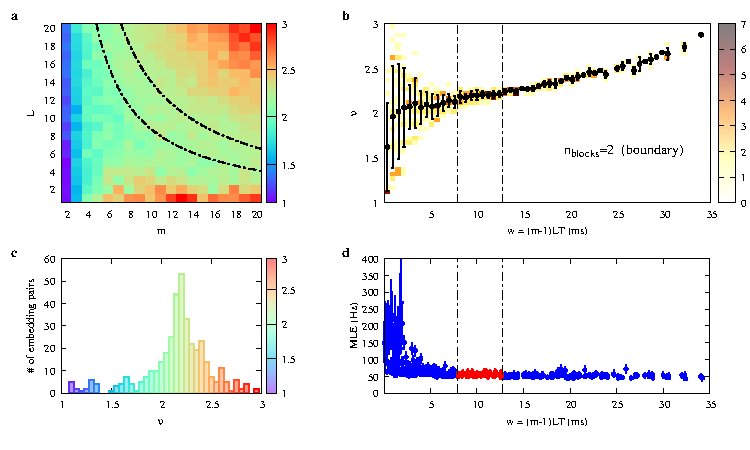
\includegraphics[width=\linewidth]{../blocks/2_blocks/1e5_points/plots/chaos.pdf}
    \caption{``Chasing chaos" analysis of the experimental $W_1$ time series obtained by setting $V_d=0.05$ V with 2 coupled blocks.
    (a) Map of estimated correlation dimension $\nu$ vs. embedding pair $(m, L)$.
    The black, dash-dotted hyperbolae bound the region of uniform $\nu$ corresponding to the interval of the
    embedding window $w$ highlighted in (b) and (d).
    (b) Sample joint distribution of $(w,\nu)$ for the $\nu$-map in (a).
    Black dots and the related errobars correspond to the expected value and the related uncertainty of $\nu$
    for each given value (bin) of $w$. A uniformity region, highlighted by the dash-dotted vertical lines,
    is identified. (c) Histogram of the estimated $\nu$. (d) Distribution of MLE as a function of $w$. Each point and the related
    uncertainty corresponds to the value assessed on an embedding pair by using the divergence rate method.
    A cluster of points, marked in red, can be identified in the uniformity region of (b), also highlighted here.}
    \label{fig:2 blocks chaos}
\end{figure}


%{Three blocks}

\begin{figure}[H]
    \centering
    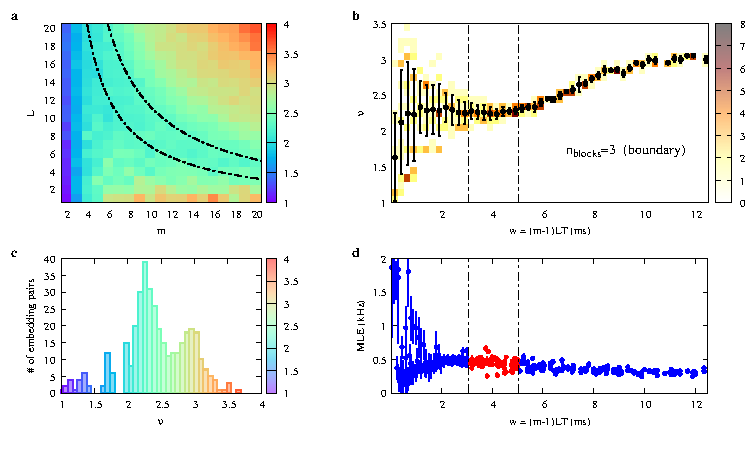
\includegraphics[width=\linewidth]{../blocks/3_blocks/edge/2e5_points/plots/chaos_low.pdf}
    \caption{``Chasing chaos" analysis of the experimental $W_1$ time series obtained by setting $V_d=0.05$ V with 3 coupled blocks.
    (a) Map of estimated correlation dimension $\nu$ vs. embedding pair $(m, L)$.
    The black, dash-dotted hyperbolae bound the region of uniform $\nu$ corresponding to the interval of the
    embedding window $w$ highlighted in (b) and (d).
    (b) Sample joint distribution of $(w,\nu)$ for the $\nu$-map in (a).
    Black dots and the related errobars correspond to the expected value and the related uncertainty of $\nu$
    for each given value (bin) of $w$. A uniformity region, highlighted by the dash-dotted vertical lines,
    is identified. (c) Histogram of the estimated $\nu$. (d) Distribution of MLE as a function of $w$. Each point and the related
    uncertainty corresponds to the value assessed on an embedding pair by using the divergence rate method.
    A cluster of points, marked in red, can be identified in the uniformity region of (b), also highlighted here.}
    \label{fig:3 blocks chaos}
\end{figure}

\begin{figure}[H]
    \centering
    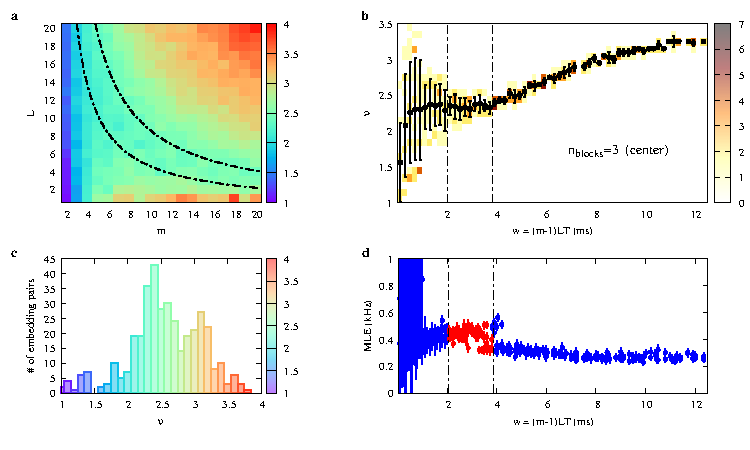
\includegraphics[width=\linewidth]{../blocks/3_blocks/middle/2e5_points/plots/chaos_low.pdf}
    \caption{``Chasing chaos" analysis of the experimental $W_2$ time series obtained by setting $V_d=0.05$ V with 3 coupled blocks.
    (a) Map of estimated correlation dimension $\nu$ vs. embedding pair $(m, L)$.
    The black, dash-dotted hyperbolae bound the region of uniform $\nu$ corresponding to the interval of the
    embedding window $w$ highlighted in (b) and (d).
    (b) Sample joint distribution of $(w,\nu)$ for the $\nu$-map in (a).
    Black dots and the related errobars correspond to the expected value and the related uncertainty of $\nu$
    for each given value (bin) of $w$. A uniformity region, highlighted by the dash-dotted vertical lines,
    is identified. (c) Histogram of the estimated $\nu$. (d) Distribution of MLE as a function of $w$. Each point and the related
    uncertainty corresponds to the value assessed on an embedding pair by using the divergence rate method.
    A cluster of points, marked in red, can be identified in the uniformity region of (b), also highlighted here.}
    \label{fig:3 blocks chaos middle}
\end{figure}

%{Four blocks}

\begin{figure}[H]
    \centering
    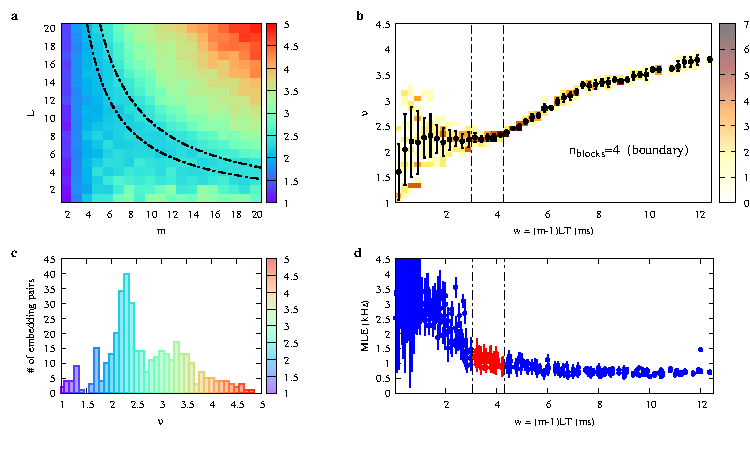
\includegraphics[width=\linewidth]{../blocks/4_blocks/2e5_points_new/plots/chaos_low.pdf}
    \caption{``Chasing chaos" analysis of the experimental $W_1$ time series obtained by setting $V_d=0.05$ V with 4 coupled blocks.
    (a) Map of estimated correlation dimension $\nu$ vs. embedding pair $(m, L)$.
    The black, dash-dotted hyperbolae bound the region of uniform $\nu$ corresponding to the interval of the
    embedding window $w$ highlighted in (b) and (d).
    (b) Sample joint distribution of $(w,\nu)$ for the $\nu$-map in (a).
    Black dots and the related errobars correspond to the expected value and the related uncertainty of $\nu$
    for each given value (bin) of $w$. A uniformity region, highlighted by the dash-dotted vertical lines,
    is identified. (c) Histogram of the estimated $\nu$. (d) Distribution of MLE as a function of $w$. Each point and the related
    uncertainty corresponds to the value assessed on an embedding pair by using the divergence rate method.
    A cluster of points, marked in red, can be identified in the uniformity region of (b), also highlighted here.}
    \label{fig:4 blocks chaos}
\end{figure}


%{Five blocks}

\begin{figure}[H]
    \centering
    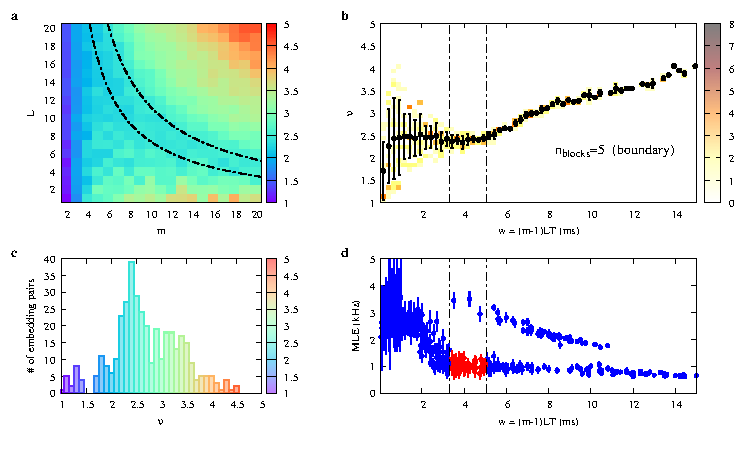
\includegraphics[width=\linewidth]{../blocks/5_blocks/edge/2e5_points/plots/chaos_low.pdf}
    \caption{``Chasing chaos" analysis of the experimental $W_1$ time series obtained by setting $V_d=0.05$ V with 5 coupled blocks.
    (a) Map of estimated correlation dimension $\nu$ vs. embedding pair $(m, L)$.
    The black, dash-dotted hyperbolae bound the region of uniform $\nu$ corresponding to the interval of the
    embedding window $w$ highlighted in (b) and (d).
    (b) Sample joint distribution of $(w,\nu)$ for the $\nu$-map in (a).
    Black dots and the related errobars correspond to the expected value and the related uncertainty of $\nu$
    for each given value (bin) of $w$. A uniformity region, highlighted by the dash-dotted vertical lines,
    is identified. (c) Histogram of the estimated $\nu$. (d) Distribution of MLE as a function of $w$. Each point and the related
    uncertainty corresponds to the value assessed on an embedding pair by using the divergence rate method.
    A cluster of points, marked in red, can be identified in the uniformity region of (b), also highlighted here.}
    \label{fig:5 blocks chaos}
\end{figure}

\begin{figure}[H]
    \centering
    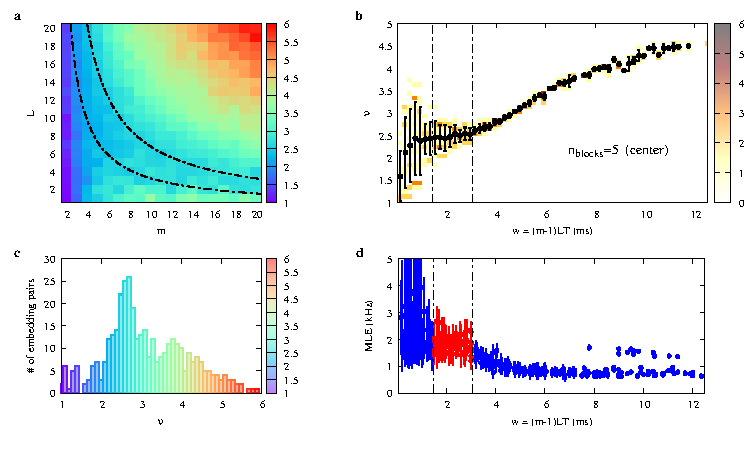
\includegraphics[width=\linewidth]{../blocks/5_blocks/middle/2e5_points/plots/chaos_low.pdf}
    \caption{``Chasing chaos" analysis of the experimental $W_3$ time series obtained by setting $V_d=0.05$ V with 5 coupled blocks.
    (a) Map of estimated correlation dimension $\nu$ vs. embedding pair $(m, L)$.
    The black, dash-dotted hyperbolae bound the region of uniform $\nu$ corresponding to the interval of the
    embedding window $w$ highlighted in (b) and (d).
    (b) Sample joint distribution of $(w,\nu)$ for the $\nu$-map in (a).
    Black dots and the related errobars correspond to the expected value and the related uncertainty of $\nu$
    for each given value (bin) of $w$. A uniformity region, highlighted by the dash-dotted vertical lines,
    is identified. (c) Histogram of the estimated $\nu$. (d) Distribution of MLE as a function of $w$. Each point and the related
    uncertainty corresponds to the value assessed on an embedding pair by using the divergence rate method.
    A cluster of points, marked in red, can be identified in the uniformity region of (b), also highlighted here.}
    \label{fig:5 blocks chaos middle}
\end{figure}

%{Six blocks}

\begin{figure}[H]
    \centering
    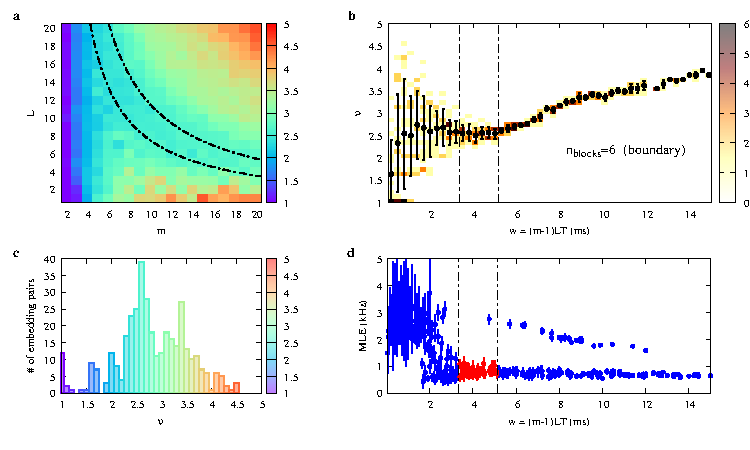
\includegraphics[width=\linewidth]{../blocks/6_blocks/2e5_points/plots/chaos_low.pdf}
    \caption{``Chasing chaos" analysis of the experimental $W_1$ time series obtained by setting $V_d=0.05$ V with 6 coupled blocks.
    (a) Map of estimated correlation dimension $\nu$ vs. embedding pair $(m, L)$.
    The black, dash-dotted hyperbolae bound the region of uniform $\nu$ corresponding to the interval of the
    embedding window $w$ highlighted in (b) and (d).
    (b) Sample joint distribution of $(w,\nu)$ for the $\nu$-map in (a).
    Black dots and the related errobars correspond to the expected value and the related uncertainty of $\nu$
    for each given value (bin) of $w$. A uniformity region, highlighted by the dash-dotted vertical lines,
    is identified. (c) Histogram of the estimated $\nu$. (d) Distribution of MLE as a function of $w$. Each point and the related
    uncertainty corresponds to the value assessed on an embedding pair by using the divergence rate method.
    A cluster of points, marked in red, can be identified in the uniformity region of (b), also highlighted here.}
    \label{fig:6 blocks chaos}
\end{figure}

%{Seven blocks}

\begin{figure}[H]
    \centering
    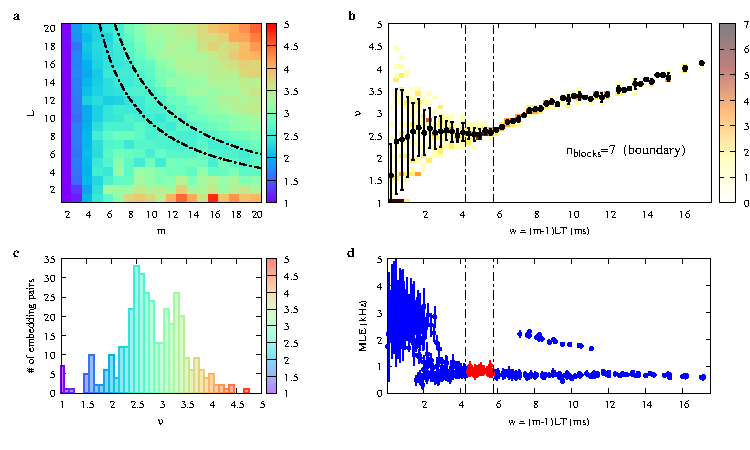
\includegraphics[width=\linewidth]{../blocks/7_blocks/edge/2e5_points/plots/chaos_low.pdf}
    \caption{``Chasing chaos" analysis of the experimental $W_1$ time series obtained by setting $V_d=0.05$ V with 7 coupled blocks.
    (a) Map of estimated correlation dimension $\nu$ vs. embedding pair $(m, L)$.
    The black, dash-dotted hyperbolae bound the region of uniform $\nu$ corresponding to the interval of the
    embedding window $w$ highlighted in (b) and (d).
    (b) Sample joint distribution of $(w,\nu)$ for the $\nu$-map in (a).
    Black dots and the related errobars correspond to the expected value and the related uncertainty of $\nu$
    for each given value (bin) of $w$. A uniformity region, highlighted by the dash-dotted vertical lines,
    is identified. (c) Histogram of the estimated $\nu$. (d) Distribution of MLE as a function of $w$. Each point and the related
    uncertainty corresponds to the value assessed on an embedding pair by using the divergence rate method.
    A cluster of points, marked in red, can be identified in the uniformity region of (b), also highlighted here.}
    \label{fig:7 blocks chaos}
\end{figure}

\begin{figure}[H]
    \centering
    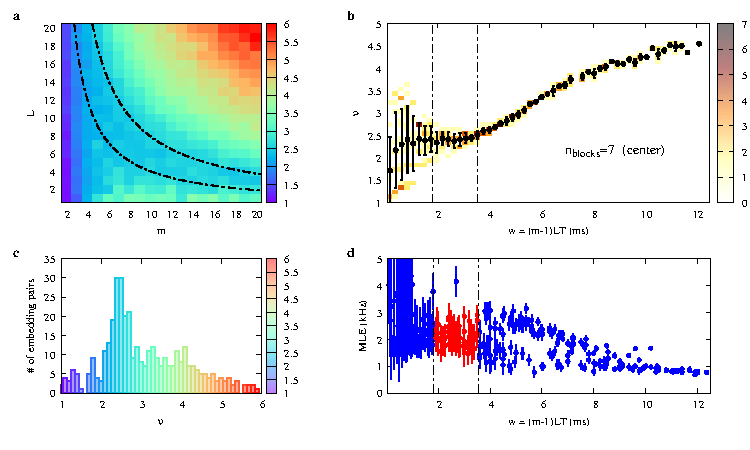
\includegraphics[width=\linewidth]{../blocks/7_blocks/middle/2e5_points/plots/chaos_low.pdf}
    \caption{``Chasing chaos" analysis of the experimental $W_4$ time series obtained by setting $V_d=0.05$ V with 7 coupled blocks.
    (a) Map of estimated correlation dimension $\nu$ vs. embedding pair $(m, L)$.
    The black, dash-dotted hyperbolae bound the region of uniform $\nu$ corresponding to the interval of the
    embedding window $w$ highlighted in (b) and (d).
    (b) Sample joint distribution of $(w,\nu)$ for the $\nu$-map in (a).
    Black dots and the related errobars correspond to the expected value and the related uncertainty of $\nu$
    for each given value (bin) of $w$. A uniformity region, highlighted by the dash-dotted vertical lines,
    is identified. (c) Histogram of the estimated $\nu$. (d) Distribution of MLE as a function of $w$. Each point and the related
    uncertainty corresponds to the value assessed on an embedding pair by using the divergence rate method.
    A cluster of points, marked in red, can be identified in the uniformity region of (b), also highlighted here.}
    \label{fig:7 blocks chaos middle}
\end{figure}

%{Eight blocks}

\begin{figure}[H]
    \centering
    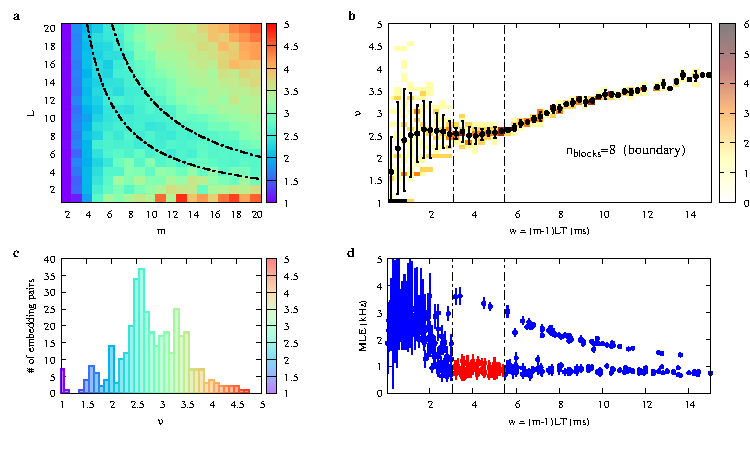
\includegraphics[width=\linewidth]{../blocks/8_blocks/2e5_points/plots/chaos_low.pdf}
    \caption{``Chasing chaos" analysis of the experimental $W_1$ time series obtained by setting $V_d=0.05$ V with 8 coupled blocks.
    (a) Map of estimated correlation dimension $\nu$ vs. embedding pair $(m, L)$.
    The black, dash-dotted hyperbolae bound the region of uniform $\nu$ corresponding to the interval of the
    embedding window $w$ highlighted in (b) and (d).
    (b) Sample joint distribution of $(w,\nu)$ for the $\nu$-map in (a).
    Black dots and the related errobars correspond to the expected value and the related uncertainty of $\nu$
    for each given value (bin) of $w$. A uniformity region, highlighted by the dash-dotted vertical lines,
    is identified. (c) Histogram of the estimated $\nu$. (d) Distribution of MLE as a function of $w$. Each point and the related
    uncertainty corresponds to the value assessed on an embedding pair by using the divergence rate method.
    A cluster of points, marked in red, can be identified in the uniformity region of (b), also highlighted here.}
    \label{fig:8 blocks chaos}
\end{figure}

%{Nine blocks}

\begin{figure}[H]
    \centering
    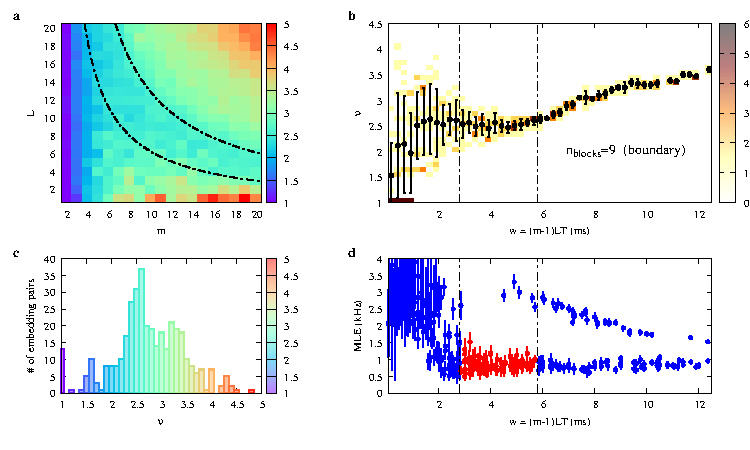
\includegraphics[width=\linewidth]{../blocks/9_blocks/edge/2e5_points/plots/chaos_low.pdf}
    \caption{``Chasing chaos" analysis of the experimental $W_1$ time series obtained by setting $V_d=0.05$ V with 9 coupled blocks.
    (a) Map of estimated correlation dimension $\nu$ vs. embedding pair $(m, L)$.
    The black, dash-dotted hyperbolae bound the region of uniform $\nu$ corresponding to the interval of the
    embedding window $w$ highlighted in (b) and (d).
    (b) Sample joint distribution of $(w,\nu)$ for the $\nu$-map in (a).
    Black dots and the related errobars correspond to the expected value and the related uncertainty of $\nu$
    for each given value (bin) of $w$. A uniformity region, highlighted by the dash-dotted vertical lines,
    is identified. (c) Histogram of the estimated $\nu$. (d) Distribution of MLE as a function of $w$. Each point and the related
    uncertainty corresponds to the value assessed on an embedding pair by using the divergence rate method.
    A cluster of points, marked in red, can be identified in the uniformity region of (b), also highlighted here.}
    \label{fig:9 blocks chaos}
\end{figure}

\begin{figure}[H]
    \centering
    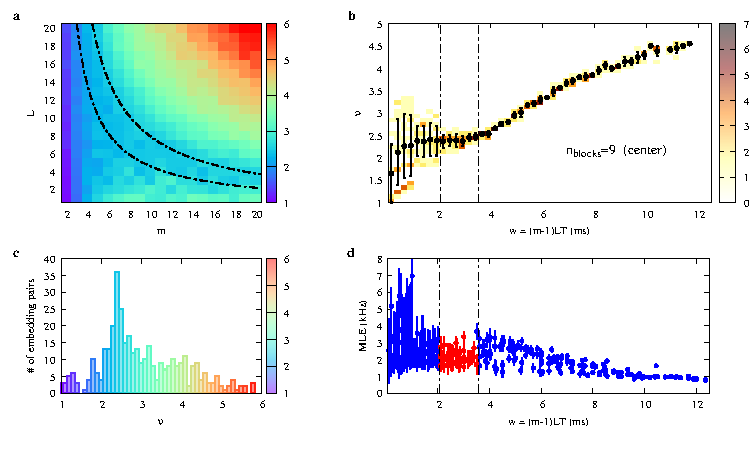
\includegraphics[width=\linewidth]{../blocks/9_blocks/middle/2e5_points/plots/chaos_low.pdf}
    \caption{``Chasing chaos" analysis of the experimental $W_5$ time series obtained by setting $V_d=0.05$ V with 9 coupled blocks.
    (a) Map of estimated correlation dimension $\nu$ vs. embedding pair $(m, L)$.
    The black, dash-dotted hyperbolae bound the region of uniform $\nu$ corresponding to the interval of the
    embedding window $w$ highlighted in (b) and (d).
    (b) Sample joint distribution of $(w,\nu)$ for the $\nu$-map in (a).
    Black dots and the related errobars correspond to the expected value and the related uncertainty of $\nu$
    for each given value (bin) of $w$. A uniformity region, highlighted by the dash-dotted vertical lines,
    is identified. (c) Histogram of the estimated $\nu$. (d) Distribution of MLE as a function of $w$. Each point and the related
    uncertainty corresponds to the value assessed on an embedding pair by using the divergence rate method.
    A cluster of points, marked in red, can be identified in the uniformity region of (b), also highlighted here.}
    \label{fig:9 blocks chaos middle}
\end{figure}

%{Ten blocks}

\begin{figure}[H]
    \centering
    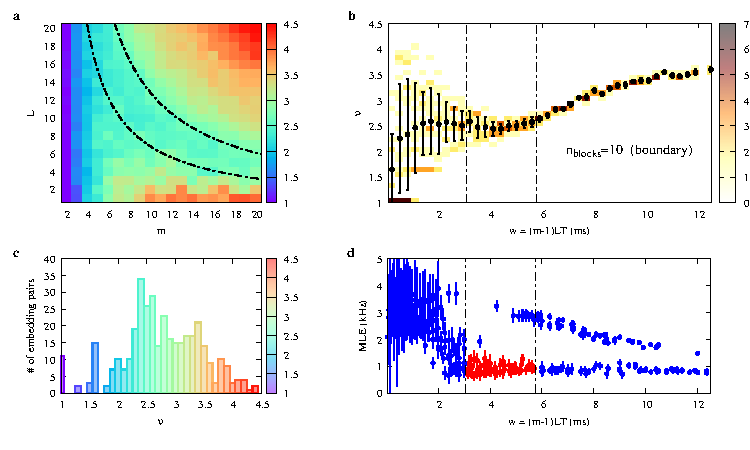
\includegraphics[width=\linewidth]{../blocks/10_blocks/2e5_points/plots/chaos_low.pdf}
    \caption{``Chasing chaos" analysis of the experimental $W_1$ time series obtained by setting $V_d=0.05$ V with 10 coupled blocks.
    (a) Map of estimated correlation dimension $\nu$ vs. embedding pair $(m, L)$.
    The black, dash-dotted hyperbolae bound the region of uniform $\nu$ corresponding to the interval of the
    embedding window $w$ highlighted in (b) and (d).
    (b) Sample joint distribution of $(w,\nu)$ for the $\nu$-map in (a).
    Black dots and the related errobars correspond to the expected value and the related uncertainty of $\nu$
    for each given value (bin) of $w$. A uniformity region, highlighted by the dash-dotted vertical lines,
    is identified. (c) Histogram of the estimated $\nu$. (d) Distribution of MLE as a function of $w$. Each point and the related
    uncertainty corresponds to the value assessed on an embedding pair by using the divergence rate method.
    A cluster of points, marked in red, can be identified in the uniformity region of (b), also highlighted here.}
    \label{fig:10 blocks chaos}
\end{figure}

%{Eleven blocks}

\begin{figure}[H]
    \centering
    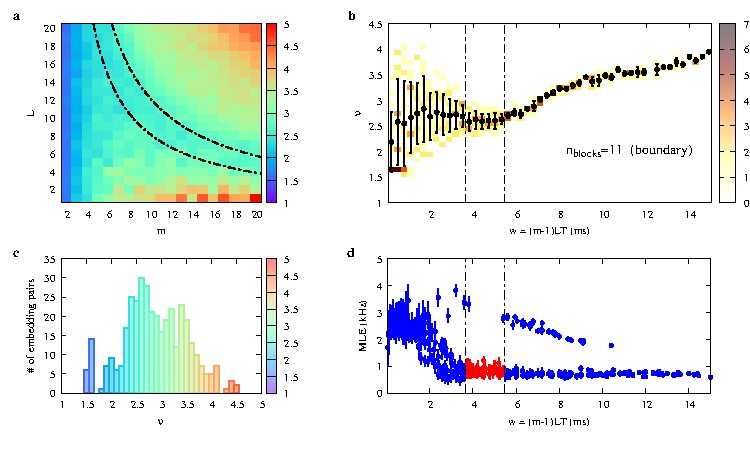
\includegraphics[width=\linewidth]{../blocks/11_blocks/edge/2e5_points/plots/chaos_low.pdf}
    \caption{``Chasing chaos" analysis of the experimental $W_1$ time series obtained by setting $V_d=0.05$ V with 11 coupled blocks.
    (a) Map of estimated correlation dimension $\nu$ vs. embedding pair $(m, L)$.
    The black, dash-dotted hyperbolae bound the region of uniform $\nu$ corresponding to the interval of the
    embedding window $w$ highlighted in (b) and (d).
    (b) Sample joint distribution of $(w,\nu)$ for the $\nu$-map in (a).
    Black dots and the related errobars correspond to the expected value and the related uncertainty of $\nu$
    for each given value (bin) of $w$. A uniformity region, highlighted by the dash-dotted vertical lines,
    is identified. (c) Histogram of the estimated $\nu$. (d) Distribution of MLE as a function of $w$. Each point and the related
    uncertainty corresponds to the value assessed on an embedding pair by using the divergence rate method.
    A cluster of points, marked in red, can be identified in the uniformity region of (b), also highlighted here.}
    \label{fig:11 blocks chaos}
\end{figure}

\begin{figure}[H]
    \centering
    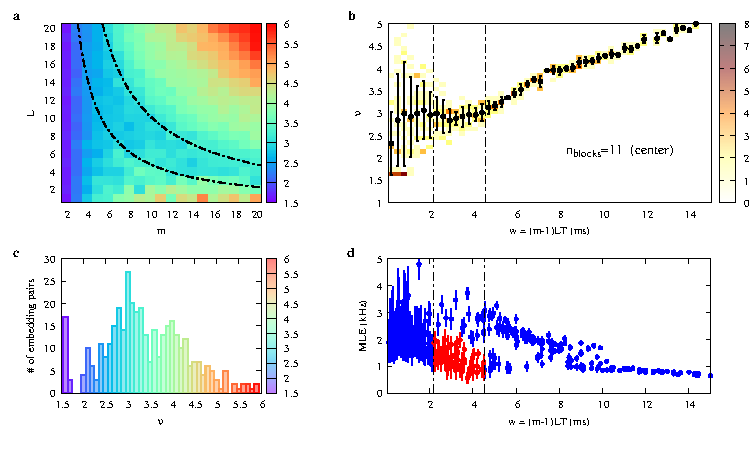
\includegraphics[width=\linewidth]{../blocks/11_blocks/middle/2e5_points/plots/chaos_low.pdf}
    \caption{``Chasing chaos" analysis of the experimental $W_6$ time series obtained by setting $V_d=0.05$ V with 11 coupled blocks.
    (a) Map of estimated correlation dimension $\nu$ vs. embedding pair $(m, L)$.
    The black, dash-dotted hyperbolae bound the region of uniform $\nu$ corresponding to the interval of the
    embedding window $w$ highlighted in (b) and (d).
    (b) Sample joint distribution of $(w,\nu)$ for the $\nu$-map in (a).
    Black dots and the related errobars correspond to the expected value and the related uncertainty of $\nu$
    for each given value (bin) of $w$. A uniformity region, highlighted by the dash-dotted vertical lines,
    is identified. (c) Histogram of the estimated $\nu$. (d) Distribution of MLE as a function of $w$. Each point and the related
    uncertainty corresponds to the value assessed on an embedding pair by using the divergence rate method.
    A cluster of points, marked in red, can be identified in the uniformity region of (b), also highlighted here.}
    \label{fig:11 blocks chaos middle}
\end{figure}

%{Twelve blocks}

\begin{figure}[H]
    \centering
    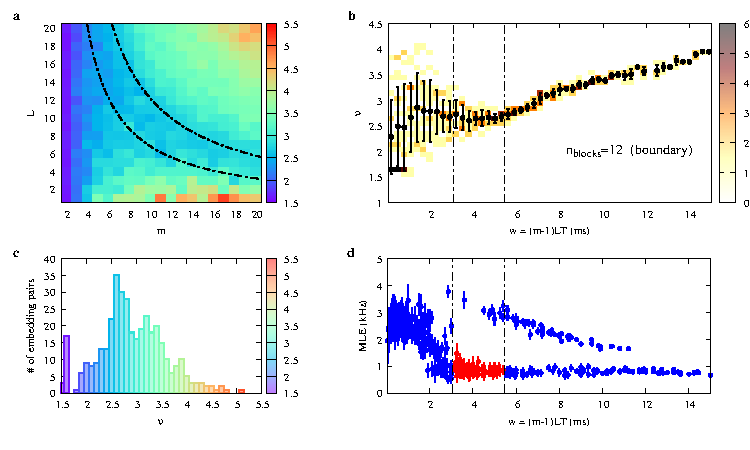
\includegraphics[width=\linewidth]{../blocks/12_blocks/2e5_points/plots/chaos_low.pdf}
    \caption{``Chasing chaos" analysis of the experimental $W_1$ time series obtained by setting $V_d=0.05$ V with 12 coupled blocks.
    (a) Map of estimated correlation dimension $\nu$ vs. embedding pair $(m, L)$.
    The black, dash-dotted hyperbolae bound the region of uniform $\nu$ corresponding to the interval of the
    embedding window $w$ highlighted in (b) and (d).
    (b) Sample joint distribution of $(w,\nu)$ for the $\nu$-map in (a).
    Black dots and the related errobars correspond to the expected value and the related uncertainty of $\nu$
    for each given value (bin) of $w$. A uniformity region, highlighted by the dash-dotted vertical lines,
    is identified. (c) Histogram of the estimated $\nu$. (d) Distribution of MLE as a function of $w$. Each point and the related
    uncertainty corresponds to the value assessed on an embedding pair by using the divergence rate method.
    A cluster of points, marked in red, can be identified in the uniformity region of (b), also highlighted here.}
    \label{fig:12 blocks chaos}
\end{figure}

%{Thirteen blocks}

\begin{figure}[H]
    \centering
    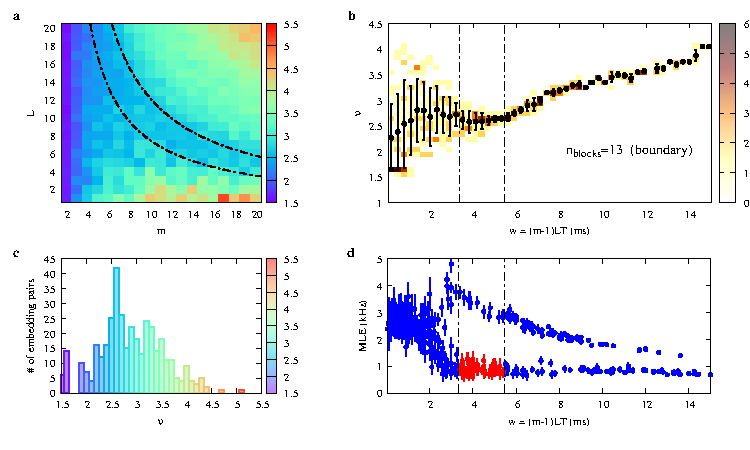
\includegraphics[width=\linewidth]{../blocks/13_blocks/edge/2e5_points/plots/chaos_low.pdf}
    \caption{``Chasing chaos" analysis of the experimental $W_1$ time series obtained by setting $V_d=0.05$ V with 13 coupled blocks.
    (a) Map of estimated correlation dimension $\nu$ vs. embedding pair $(m, L)$.
    The black, dash-dotted hyperbolae bound the region of uniform $\nu$ corresponding to the interval of the
    embedding window $w$ highlighted in (b) and (d).
    (b) Sample joint distribution of $(w,\nu)$ for the $\nu$-map in (a).
    Black dots and the related errobars correspond to the expected value and the related uncertainty of $\nu$
    for each given value (bin) of $w$. A uniformity region, highlighted by the dash-dotted vertical lines,
    is identified. (c) Histogram of the estimated $\nu$. (d) Distribution of MLE as a function of $w$. Each point and the related
    uncertainty corresponds to the value assessed on an embedding pair by using the divergence rate method.
    A cluster of points, marked in red, can be identified in the uniformity region of (b), also highlighted here.}
    \label{fig:13 blocks chaos}
\end{figure}

\begin{figure}[H]
    \centering
    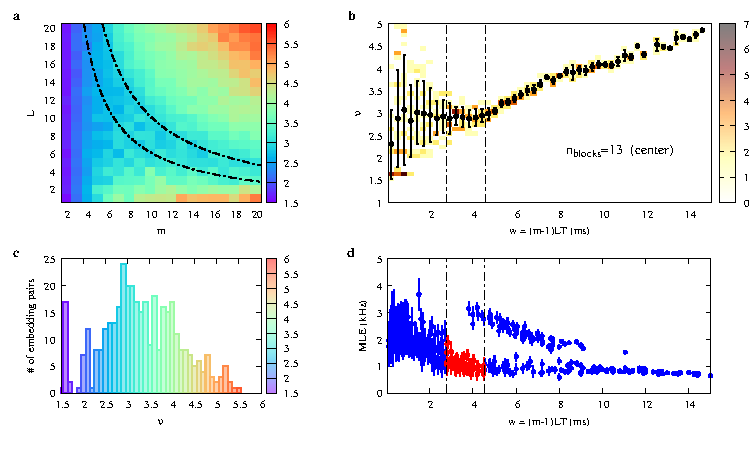
\includegraphics[width=\linewidth]{../blocks/13_blocks/middle/2e5_points/plots/chaos_low.pdf}
    \caption{``Chasing chaos" analysis of the experimental $W_7$ time series obtained by setting $V_d=0.05$ V with 13 coupled blocks.
    (a) Map of estimated correlation dimension $\nu$ vs. embedding pair $(m, L)$.
    The black, dash-dotted hyperbolae bound the region of uniform $\nu$ corresponding to the interval of the
    embedding window $w$ highlighted in (b) and (d).
    (b) Sample joint distribution of $(w,\nu)$ for the $\nu$-map in (a).
    Black dots and the related errobars correspond to the expected value and the related uncertainty of $\nu$
    for each given value (bin) of $w$. A uniformity region, highlighted by the dash-dotted vertical lines,
    is identified. (c) Histogram of the estimated $\nu$. (d) Distribution of MLE as a function of $w$. Each point and the related
    uncertainty corresponds to the value assessed on an embedding pair by using the divergence rate method.
    A cluster of points, marked in red, can be identified in the uniformity region of (b), also highlighted here.}
    \label{fig:13 blocks chaos middle}
\end{figure}

%{Fourteen blocks}

\begin{figure}[H]
    \centering
    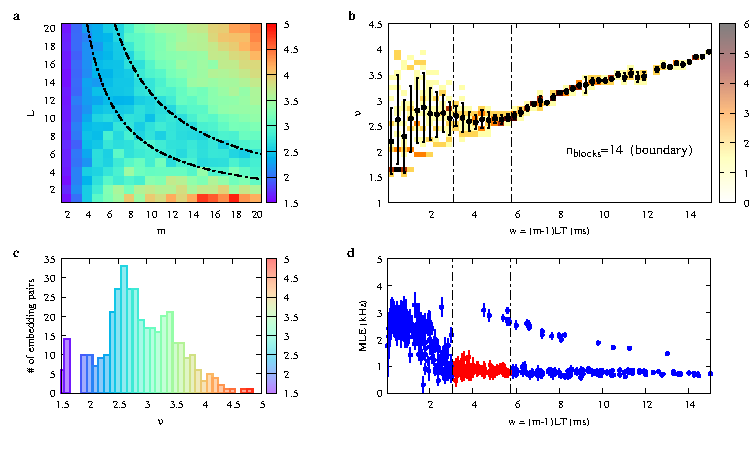
\includegraphics[width=\linewidth]{../blocks/14_blocks/2e5_points/plots/chaos_low.pdf}
    \caption{``Chasing chaos" analysis of the experimental $W_1$ time series obtained by setting $V_d=0.05$ V with 14 coupled blocks.
    (a) Map of estimated correlation dimension $\nu$ vs. embedding pair $(m, L)$.
    The black, dash-dotted hyperbolae bound the region of uniform $\nu$ corresponding to the interval of the
    embedding window $w$ highlighted in (b) and (d).
    (b) Sample joint distribution of $(w,\nu)$ for the $\nu$-map in (a).
    Black dots and the related errobars correspond to the expected value and the related uncertainty of $\nu$
    for each given value (bin) of $w$. A uniformity region, highlighted by the dash-dotted vertical lines,
    is identified. (c) Histogram of the estimated $\nu$. (d) Distribution of MLE as a function of $w$. Each point and the related
    uncertainty corresponds to the value assessed on an embedding pair by using the divergence rate method.
    A cluster of points, marked in red, can be identified in the uniformity region of (b), also highlighted here.}
    \label{fig:14 blocks chaos}
\end{figure}

%{Fifteen blocks}

\begin{figure}[H]
    \centering
    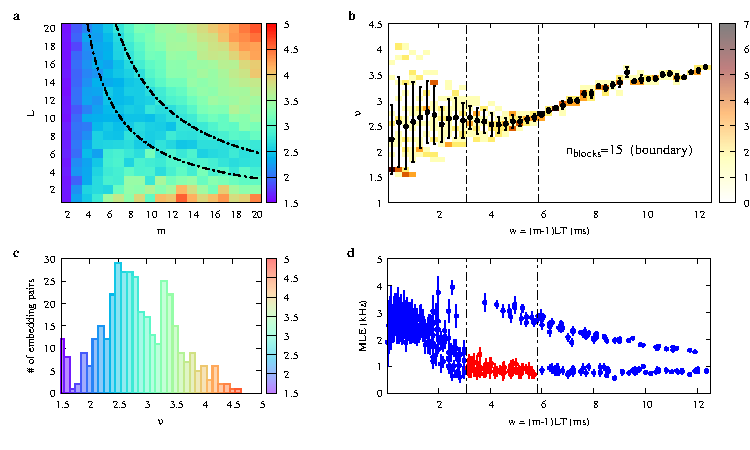
\includegraphics[width=\linewidth]{../blocks/15_blocks/edge/2e5_points/plots/chaos_low.pdf}
    \caption{``Chasing chaos" analysis of the experimental $W_1$ time series obtained by setting $V_d=0.05$ V with 15 coupled blocks.
    (a) Map of estimated correlation dimension $\nu$ vs. embedding pair $(m, L)$.
    The black, dash-dotted hyperbolae bound the region of uniform $\nu$ corresponding to the interval of the
    embedding window $w$ highlighted in (b) and (d).
    (b) Sample joint distribution of $(w,\nu)$ for the $\nu$-map in (a).
    Black dots and the related errobars correspond to the expected value and the related uncertainty of $\nu$
    for each given value (bin) of $w$. A uniformity region, highlighted by the dash-dotted vertical lines,
    is identified. (c) Histogram of the estimated $\nu$. (d) Distribution of MLE as a function of $w$. Each point and the related
    uncertainty corresponds to the value assessed on an embedding pair by using the divergence rate method.
    A cluster of points, marked in red, can be identified in the uniformity region of (b), also highlighted here.}
    \label{fig:15 blocks chaos}
\end{figure}

\begin{figure}[H]
    \centering
    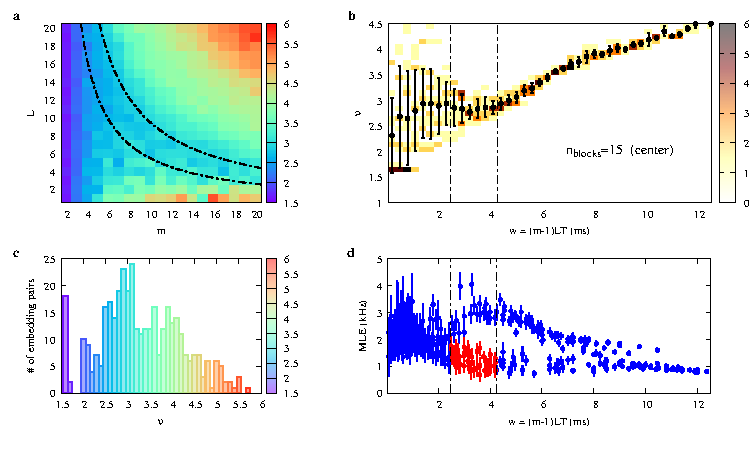
\includegraphics[width=\linewidth]{../blocks/15_blocks/middle/2e5_points/plots/chaos_low.pdf}
    \caption{``Chasing chaos" analysis of the experimental $W_8$ time series obtained by setting $V_d=0.05$ V with 15 coupled blocks.
    (a) Map of estimated correlation dimension $\nu$ vs. embedding pair $(m, L)$.
    The black, dash-dotted hyperbolae bound the region of uniform $\nu$ corresponding to the interval of the
    embedding window $w$ highlighted in (b) and (d).
    (b) Sample joint distribution of $(w,\nu)$ for the $\nu$-map in (a).
    Black dots and the related errobars correspond to the expected value and the related uncertainty of $\nu$
    for each given value (bin) of $w$. A uniformity region, highlighted by the dash-dotted vertical lines,
    is identified. (c) Histogram of the estimated $\nu$. (d) Distribution of MLE as a function of $w$. Each point and the related
    uncertainty corresponds to the value assessed on an embedding pair by using the divergence rate method.
    A cluster of points, marked in red, can be identified in the uniformity region of (b), also highlighted here.}
    \label{fig:15 blocks middle chaos}
\end{figure}

%{Sixteen blocks}

\begin{figure}[H]
    \centering
    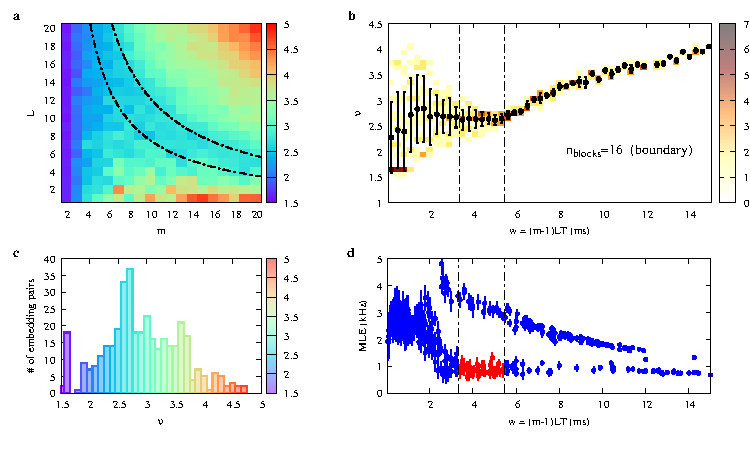
\includegraphics[width=\linewidth]{../blocks/16_blocks/2e5_points/plots/chaos_low.pdf}
    \caption{``Chasing chaos" analysis of the experimental $W_1$ time series obtained by setting $V_d=0.05$ V with 16 coupled blocks.
    (a) Map of estimated correlation dimension $\nu$ vs. embedding pair $(m, L)$.
    The black, dash-dotted hyperbolae bound the region of uniform $\nu$ corresponding to the interval of the
    embedding window $w$ highlighted in (b) and (d).
    (b) Sample joint distribution of $(w,\nu)$ for the $\nu$-map in (a).
    Black dots and the related errobars correspond to the expected value and the related uncertainty of $\nu$
    for each given value (bin) of $w$. A uniformity region, highlighted by the dash-dotted vertical lines,
    is identified. (c) Histogram of the estimated $\nu$. (d) Distribution of MLE as a function of $w$. Each point and the related
    uncertainty corresponds to the value assessed on an embedding pair by using the divergence rate method.
    A cluster of points, marked in red, can be identified in the uniformity region of (b), also highlighted here.}
    \label{fig:16 blocks chaos}
\end{figure}

%{Seventeen blocks}

\begin{figure}[H]
    \centering
    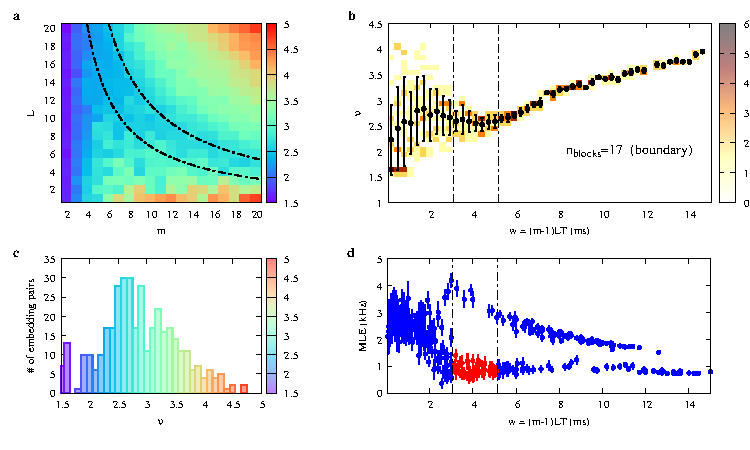
\includegraphics[width=\linewidth]{../blocks/17_blocks/edge/2e5_points/plots/chaos_low.pdf}
    \caption{``Chasing chaos" analysis of the experimental $W_1$ time series obtained by setting $V_d=0.05$ V with 17 coupled blocks.
    (a) Map of estimated correlation dimension $\nu$ vs. embedding pair $(m, L)$.
    The black, dash-dotted hyperbolae bound the region of uniform $\nu$ corresponding to the interval of the
    embedding window $w$ highlighted in (b) and (d).
    (b) Sample joint distribution of $(w,\nu)$ for the $\nu$-map in (a).
    Black dots and the related errobars correspond to the expected value and the related uncertainty of $\nu$
    for each given value (bin) of $w$. A uniformity region, highlighted by the dash-dotted vertical lines,
    is identified. (c) Histogram of the estimated $\nu$. (d) Distribution of MLE as a function of $w$. Each point and the related
    uncertainty corresponds to the value assessed on an embedding pair by using the divergence rate method.
    A cluster of points, marked in red, can be identified in the uniformity region of (b), also highlighted here.}
    \label{fig:17 blocks chaos}
\end{figure}


\begin{figure}[H]
    \centering
    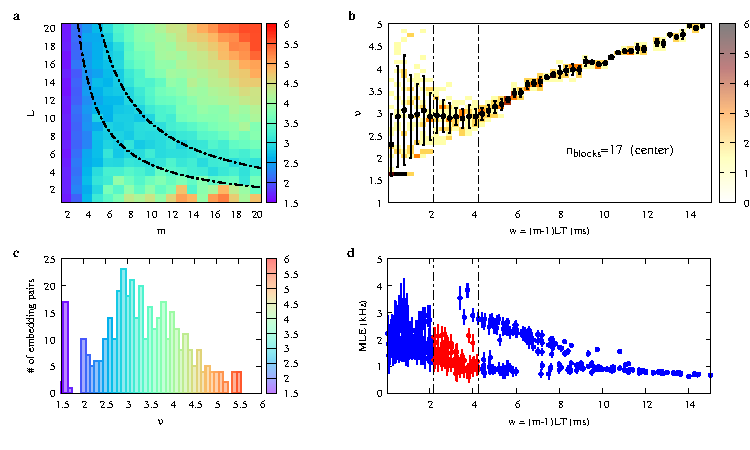
\includegraphics[width=\linewidth]{../blocks/17_blocks/middle/2e5_points/plots/chaos_low.pdf}
    \caption{``Chasing chaos" analysis of the experimental $W_9$ time series obtained by setting $V_d=0.05$ V with 17 coupled blocks.
    (a) Map of estimated correlation dimension $\nu$ vs. embedding pair $(m, L)$.
    The black, dash-dotted hyperbolae bound the region of uniform $\nu$ corresponding to the interval of the
    embedding window $w$ highlighted in (b) and (d).
    (b) Sample joint distribution of $(w,\nu)$ for the $\nu$-map in (a).
    Black dots and the related errobars correspond to the expected value and the related uncertainty of $\nu$
    for each given value (bin) of $w$. A uniformity region, highlighted by the dash-dotted vertical lines,
    is identified. (c) Histogram of the estimated $\nu$. (d) Distribution of MLE as a function of $w$. Each point and the related
    uncertainty corresponds to the value assessed on an embedding pair by using the divergence rate method.
    A cluster of points, marked in red, can be identified in the uniformity region of (b), also highlighted here.}
    \label{fig:17 blocks chaos middle}
\end{figure}

%{Eighteen blocks}

\begin{figure}[H]
    \centering
    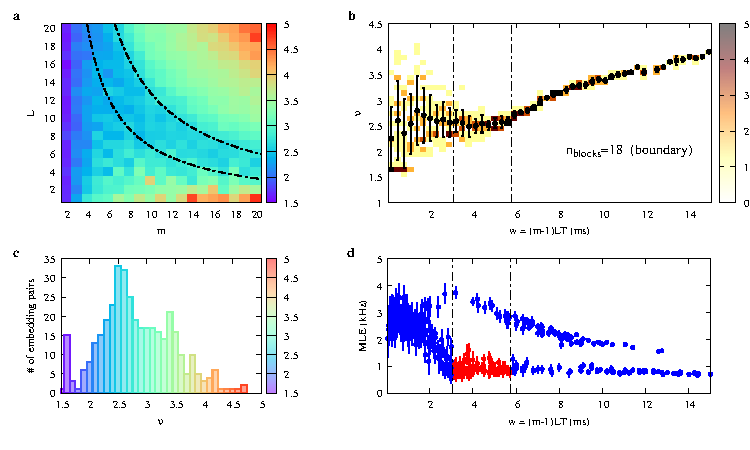
\includegraphics[width=\linewidth]{../blocks/18_blocks/2e5_points/plots/chaos_low.pdf}
    \caption{``Chasing chaos" analysis of the experimental $W_1$ time series obtained by setting $V_d=0.05$ V with 18 coupled blocks.
    (a) Map of estimated correlation dimension $\nu$ vs. embedding pair $(m, L)$.
    The black, dash-dotted hyperbolae bound the region of uniform $\nu$ corresponding to the interval of the
    embedding window $w$ highlighted in (b) and (d).
    (b) Sample joint distribution of $(w,\nu)$ for the $\nu$-map in (a).
    Black dots and the related errobars correspond to the expected value and the related uncertainty of $\nu$
    for each given value (bin) of $w$. A uniformity region, highlighted by the dash-dotted vertical lines,
    is identified. (c) Histogram of the estimated $\nu$. (d) Distribution of MLE as a function of $w$. Each point and the related
    uncertainty corresponds to the value assessed on an embedding pair by using the divergence rate method.
    A cluster of points, marked in red, can be identified in the uniformity region of (b), also highlighted here.}
    \label{fig:18 blocks chaos}
\end{figure}

%{Nineteen blocks}

\begin{figure}[H]
    \centering
    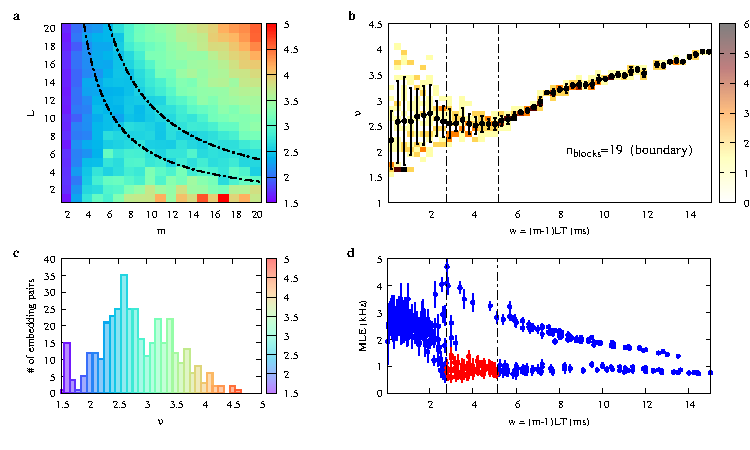
\includegraphics[width=\linewidth]{../blocks/19_blocks/edge/2e5_points/plots/chaos_low.pdf}
    \caption{``Chasing chaos" analysis of the experimental $W_1$ time series obtained by setting $V_d=0.05$ V with 19 coupled blocks.
    (a) Map of estimated correlation dimension $\nu$ vs. embedding pair $(m, L)$.
    The black, dash-dotted hyperbolae bound the region of uniform $\nu$ corresponding to the interval of the
    embedding window $w$ highlighted in (b) and (d).
    (b) Sample joint distribution of $(w,\nu)$ for the $\nu$-map in (a).
    Black dots and the related errobars correspond to the expected value and the related uncertainty of $\nu$
    for each given value (bin) of $w$. A uniformity region, highlighted by the dash-dotted vertical lines,
    is identified. (c) Histogram of the estimated $\nu$. (d) Distribution of MLE as a function of $w$. Each point and the related
    uncertainty corresponds to the value assessed on an embedding pair by using the divergence rate method.
    A cluster of points, marked in red, can be identified in the uniformity region of (b), also highlighted here.}
    \label{fig:19 blocks chaos}
\end{figure}

\begin{figure}[H]
    \centering
    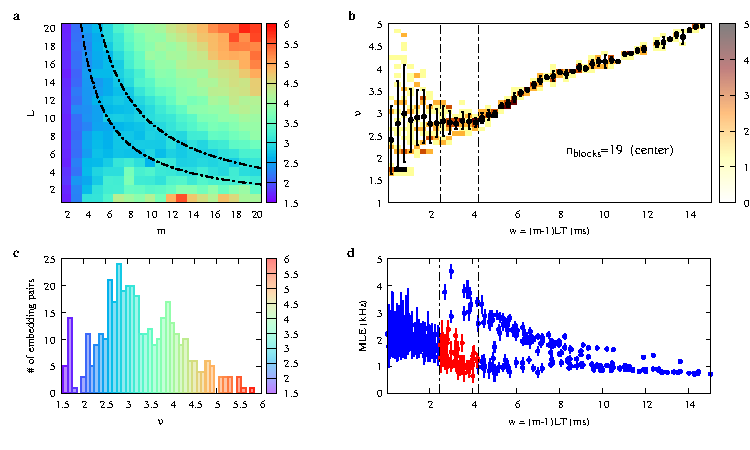
\includegraphics[width=\linewidth]{../blocks/19_blocks/middle/2e5_points/plots/chaos_low.pdf}
    \caption{``Chasing chaos" analysis of the experimental $W_{10}$ time series obtained by setting $V_d=0.05$ V with 19 coupled blocks.
    (a) Map of estimated correlation dimension $\nu$ vs. embedding pair $(m, L)$.
    The black, dash-dotted hyperbolae bound the region of uniform $\nu$ corresponding to the interval of the
    embedding window $w$ highlighted in (b) and (d).
    (b) Sample joint distribution of $(w,\nu)$ for the $\nu$-map in (a).
    Black dots and the related errobars correspond to the expected value and the related uncertainty of $\nu$
    for each given value (bin) of $w$. A uniformity region, highlighted by the dash-dotted vertical lines,
    is identified. (c) Histogram of the estimated $\nu$. (d) Distribution of MLE as a function of $w$. Each point and the related
    uncertainty corresponds to the value assessed on an embedding pair by using the divergence rate method.
    A cluster of points, marked in red, can be identified in the uniformity region of (b), also highlighted here.}
    \label{fig:19 blocks chaos middle}
\end{figure}

%{Twenty blocks}

\begin{figure}[H]
    \centering
    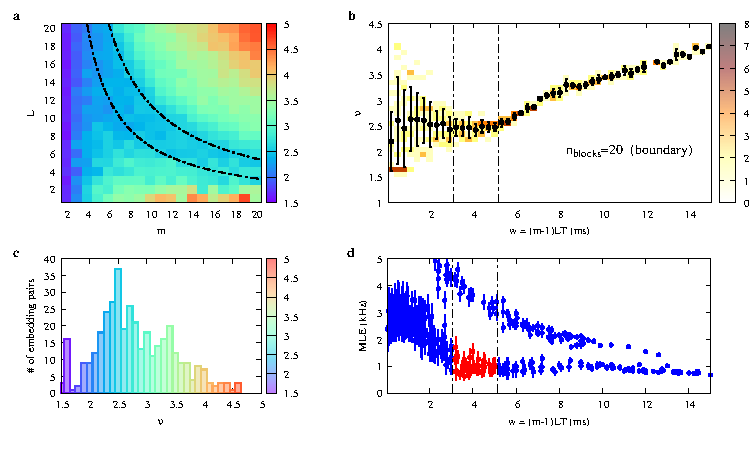
\includegraphics[width=\linewidth]{../blocks/20_blocks/2e5_points/plots/chaos_low.pdf}
    \caption{``Chasing chaos" analysis of the experimental $W_1$ time series obtained by setting $V_d=0.05$ V with 20 coupled blocks.
    (a) Map of estimated correlation dimension $\nu$ vs. embedding pair $(m, L)$.
    The black, dash-dotted hyperbolae bound the region of uniform $\nu$ corresponding to the interval of the
    embedding window $w$ highlighted in (b) and (d).
    (b) Sample joint distribution of $(w,\nu)$ for the $\nu$-map in (a).
    Black dots and the related errobars correspond to the expected value and the related uncertainty of $\nu$
    for each given value (bin) of $w$. A uniformity region, highlighted by the dash-dotted vertical lines,
    is identified. (c) Histogram of the estimated $\nu$. (d) Distribution of MLE as a function of $w$. Each point and the related
    uncertainty corresponds to the value assessed on an embedding pair by using the divergence rate method.
    A cluster of points, marked in red, can be identified in the uniformity region of (b), also highlighted here.}
    \label{fig:20 blocks chaos}
\end{figure}

%{Twentyone blocks}

\begin{figure}[H]
    \centering
    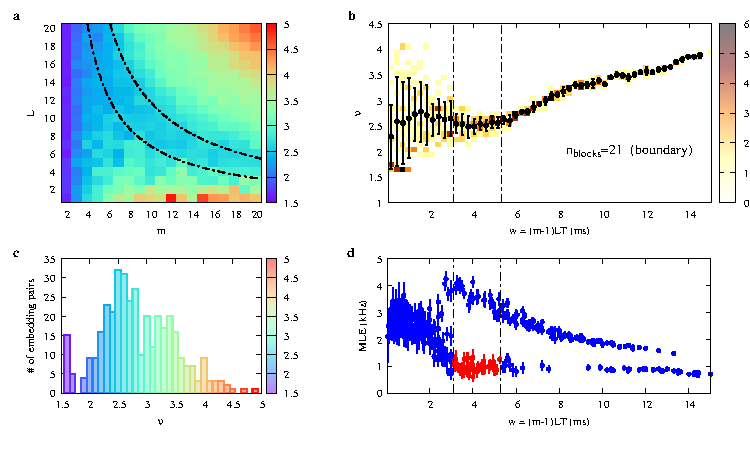
\includegraphics[width=\linewidth]{../blocks/21_blocks/edge/2e5_points/plots/chaos_low.pdf}
    \caption{``Chasing chaos" analysis of the experimental $W_1$ time series obtained by setting $V_d=0.05$ V with 21 coupled blocks.
    (a) Map of estimated correlation dimension $\nu$ vs. embedding pair $(m, L)$.
    The black, dash-dotted hyperbolae bound the region of uniform $\nu$ corresponding to the interval of the
    embedding window $w$ highlighted in (b) and (d).
    (b) Sample joint distribution of $(w,\nu)$ for the $\nu$-map in (a).
    Black dots and the related errobars correspond to the expected value and the related uncertainty of $\nu$
    for each given value (bin) of $w$. A uniformity region, highlighted by the dash-dotted vertical lines,
    is identified. (c) Histogram of the estimated $\nu$. (d) Distribution of MLE as a function of $w$. Each point and the related
    uncertainty corresponds to the value assessed on an embedding pair by using the divergence rate method.
    A cluster of points, marked in red, can be identified in the uniformity region of (b), also highlighted here.}
    \label{fig:21 blocks chaos}
\end{figure}

\begin{figure}[H]
    \centering
    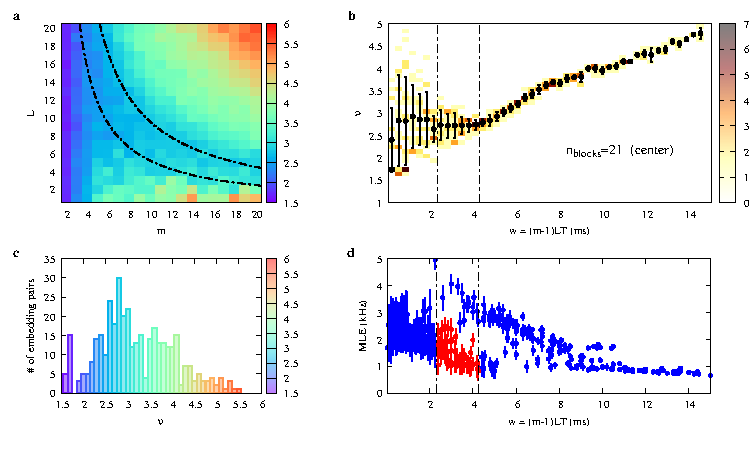
\includegraphics[width=\linewidth]{../blocks/21_blocks/middle/2e5_points/plots/chaos_low.pdf}
    \caption{``Chasing chaos" analysis of the experimental $W_{11}$ time series obtained by setting $V_d=0.05$ V with 21 coupled blocks.
    (a) Map of estimated correlation dimension $\nu$ vs. embedding pair $(m, L)$.
    The black, dash-dotted hyperbolae bound the region of uniform $\nu$ corresponding to the interval of the
    embedding window $w$ highlighted in (b) and (d).
    (b) Sample joint distribution of $(w,\nu)$ for the $\nu$-map in (a).
    Black dots and the related errobars correspond to the expected value and the related uncertainty of $\nu$
    for each given value (bin) of $w$. A uniformity region, highlighted by the dash-dotted vertical lines,
    is identified. (c) Histogram of the estimated $\nu$. (d) Distribution of MLE as a function of $w$. Each point and the related
    uncertainty corresponds to the value assessed on an embedding pair by using the divergence rate method.
    A cluster of points, marked in red, can be identified in the uniformity region of (b), also highlighted here.}
    \label{fig:21 blocks chaos middle}
\end{figure}

%{Twentytwo blocks}

\begin{figure}[H]
    \centering
    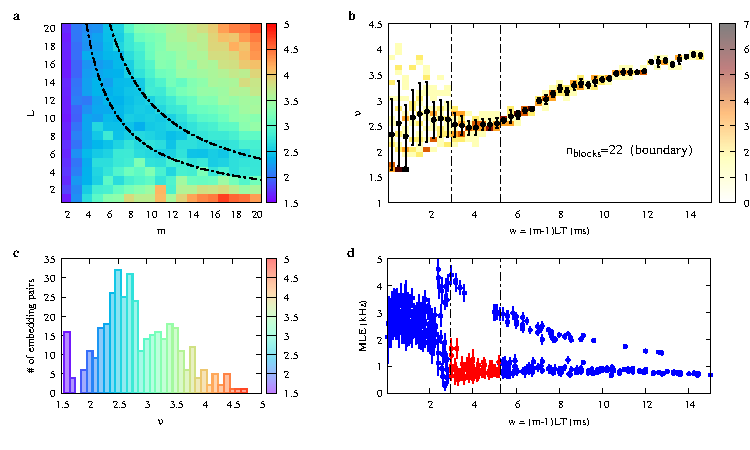
\includegraphics[width=\linewidth]{../blocks/22_blocks/2e5_points/plots/chaos_low.pdf}
    \caption{``Chasing chaos" analysis of the experimental $W_1$ time series obtained by setting $V_d=0.05$ V with 22 coupled blocks.
    (a) Map of estimated correlation dimension $\nu$ vs. embedding pair $(m, L)$.
    The black, dash-dotted hyperbolae bound the region of uniform $\nu$ corresponding to the interval of the
    embedding window $w$ highlighted in (b) and (d).
    (b) Sample joint distribution of $(w,\nu)$ for the $\nu$-map in (a).
    Black dots and the related errobars correspond to the expected value and the related uncertainty of $\nu$
    for each given value (bin) of $w$. A uniformity region, highlighted by the dash-dotted vertical lines,
    is identified. (c) Histogram of the estimated $\nu$. (d) Distribution of MLE as a function of $w$. Each point and the related
    uncertainty corresponds to the value assessed on an embedding pair by using the divergence rate method.
    A cluster of points, marked in red, can be identified in the uniformity region of (b), also highlighted here.}
    \label{fig:22 blocks chaos}
\end{figure}

%{Twentythree blocks}

\begin{figure}[H]
    \centering
    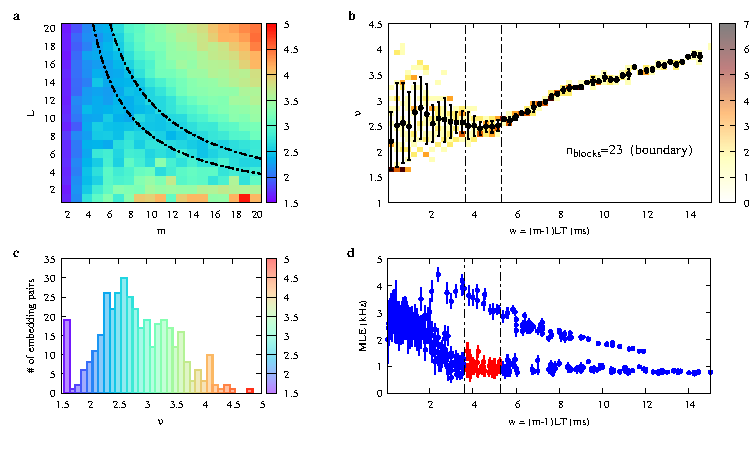
\includegraphics[width=\linewidth]{../blocks/23_blocks/edge/2e5_points/plots/chaos_low.pdf}
    \caption{``Chasing chaos" analysis of the experimental $W_1$ time series obtained by setting $V_d=0.05$ V with 23 coupled blocks.
    (a) Map of estimated correlation dimension $\nu$ vs. embedding pair $(m, L)$.
    The black, dash-dotted hyperbolae bound the region of uniform $\nu$ corresponding to the interval of the
    embedding window $w$ highlighted in (b) and (d).
    (b) Sample joint distribution of $(w,\nu)$ for the $\nu$-map in (a).
    Black dots and the related errobars correspond to the expected value and the related uncertainty of $\nu$
    for each given value (bin) of $w$. A uniformity region, highlighted by the dash-dotted vertical lines,
    is identified. (c) Histogram of the estimated $\nu$. (d) Distribution of MLE as a function of $w$. Each point and the related
    uncertainty corresponds to the value assessed on an embedding pair by using the divergence rate method.
    A cluster of points, marked in red, can be identified in the uniformity region of (b), also highlighted here.}
    \label{fig:23 blocks chaos}
\end{figure}

\begin{figure}[H]
    \centering
    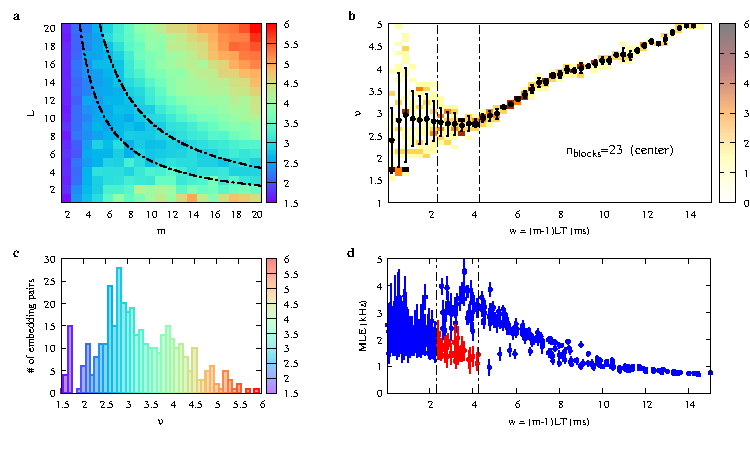
\includegraphics[width=\linewidth]{../blocks/23_blocks/middle/2e5_points/plots/chaos_low.pdf}
    \caption{``Chasing chaos" analysis of the experimental $W_{12}$ time series obtained by setting $V_d=0.05$ V with 23 coupled blocks.
    (a) Map of estimated correlation dimension $\nu$ vs. embedding pair $(m, L)$.
    The black, dash-dotted hyperbolae bound the region of uniform $\nu$ corresponding to the interval of the
    embedding window $w$ highlighted in (b) and (d).
    (b) Sample joint distribution of $(w,\nu)$ for the $\nu$-map in (a).
    Black dots and the related errobars correspond to the expected value and the related uncertainty of $\nu$
    for each given value (bin) of $w$. A uniformity region, highlighted by the dash-dotted vertical lines,
    is identified. (c) Histogram of the estimated $\nu$. (d) Distribution of MLE as a function of $w$. Each point and the related
    uncertainty corresponds to the value assessed on an embedding pair by using the divergence rate method.
    A cluster of points, marked in red, can be identified in the uniformity region of (b), also highlighted here.}
    \label{fig:23 blocks chaos middle}
\end{figure}

%{Twentyfour blocks}

\begin{figure}[H]
    \centering
    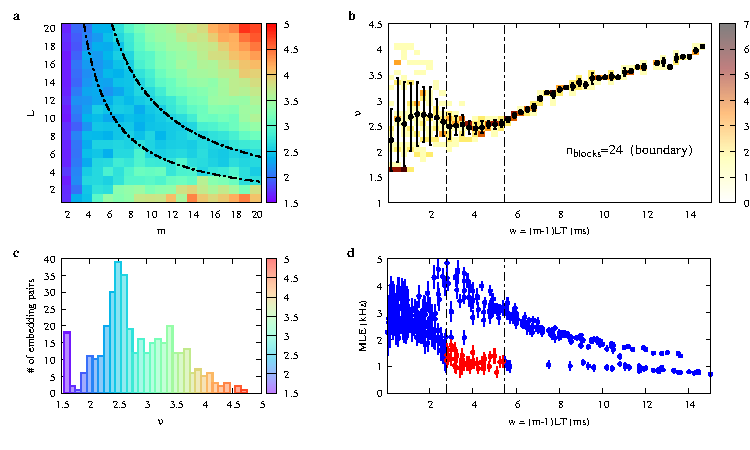
\includegraphics[width=\linewidth]{../blocks/24_blocks/2e5_points/plots/chaos_low.pdf}
    \caption{``Chasing chaos" analysis of the experimental $W_1$ time series obtained by setting $V_d=0.05$ V with 24 coupled blocks.
    (a) Map of estimated correlation dimension $\nu$ vs. embedding pair $(m, L)$.
    The black, dash-dotted hyperbolae bound the region of uniform $\nu$ corresponding to the interval of the
    embedding window $w$ highlighted in (b) and (d).
    (b) Sample joint distribution of $(w,\nu)$ for the $\nu$-map in (a).
    Black dots and the related errobars correspond to the expected value and the related uncertainty of $\nu$
    for each given value (bin) of $w$. A uniformity region, highlighted by the dash-dotted vertical lines,
    is identified. (c) Histogram of the estimated $\nu$. (d) Distribution of MLE as a function of $w$. Each point and the related
    uncertainty corresponds to the value assessed on an embedding pair by using the divergence rate method.
    A cluster of points, marked in red, can be identified in the uniformity region of (b), also highlighted here.}
    \label{fig:24 blocks chaos}
\end{figure}

%{Twentyfive blocks}

\begin{figure}[H]
    \centering
    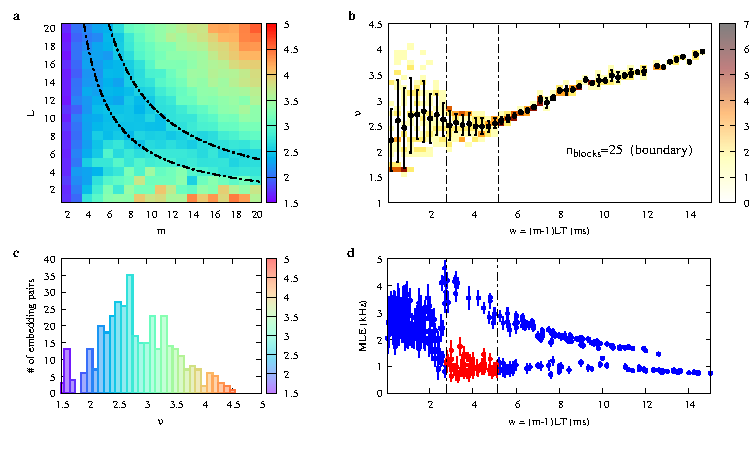
\includegraphics[width=\linewidth]{../blocks/25_blocks/edge/2e5_points/plots/chaos_low.pdf}
    \caption{``Chasing chaos" analysis of the experimental $W_1$ time series obtained by setting $V_d=0.05$ V with 25 coupled blocks.
    (a) Map of estimated correlation dimension $\nu$ vs. embedding pair $(m, L)$.
    The black, dash-dotted hyperbolae bound the region of uniform $\nu$ corresponding to the interval of the
    embedding window $w$ highlighted in (b) and (d).
    (b) Sample joint distribution of $(w,\nu)$ for the $\nu$-map in (a).
    Black dots and the related errobars correspond to the expected value and the related uncertainty of $\nu$
    for each given value (bin) of $w$. A uniformity region, highlighted by the dash-dotted vertical lines,
    is identified. (c) Histogram of the estimated $\nu$. (d) Distribution of MLE as a function of $w$. Each point and the related
    uncertainty corresponds to the value assessed on an embedding pair by using the divergence rate method.
    A cluster of points, marked in red, can be identified in the uniformity region of (b), also highlighted here.}
    \label{fig:25 blocks chaos}
\end{figure}

\begin{figure}[H]
    \centering
    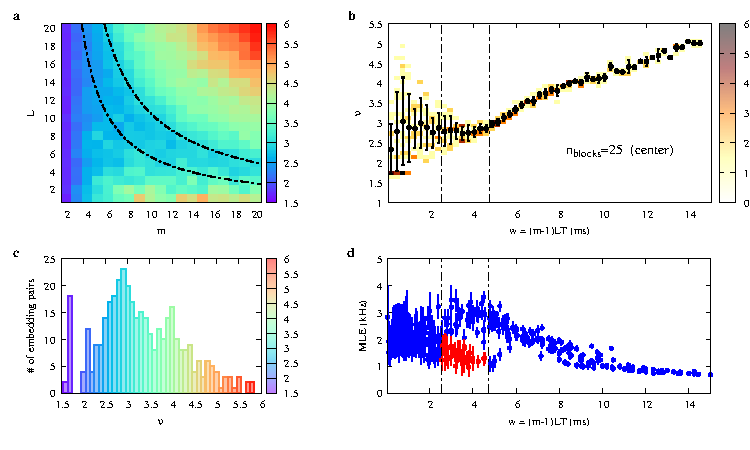
\includegraphics[width=\linewidth]{../blocks/25_blocks/middle/2e5_points/plots/chaos_low.pdf}
    \caption{``Chasing chaos" analysis of the experimental $W_{13}$ time series obtained by setting $V_d=0.05$ V with 25 coupled blocks.
    (a) Map of estimated correlation dimension $\nu$ vs. embedding pair $(m, L)$.
    The black, dash-dotted hyperbolae bound the region of uniform $\nu$ corresponding to the interval of the
    embedding window $w$ highlighted in (b) and (d).
    (b) Sample joint distribution of $(w,\nu)$ for the $\nu$-map in (a).
    Black dots and the related errobars correspond to the expected value and the related uncertainty of $\nu$
    for each given value (bin) of $w$. A uniformity region, highlighted by the dash-dotted vertical lines,
    is identified. (c) Histogram of the estimated $\nu$. (d) Distribution of MLE as a function of $w$. Each point and the related
    uncertainty corresponds to the value assessed on an embedding pair by using the divergence rate method.
    A cluster of points, marked in red, can be identified in the uniformity region of (b), also highlighted here.}
    \label{fig:25 blocks chaos middle}
\end{figure}

\clearpage

\section{Conclusions}

\begin{figure}[H]
    \centering
    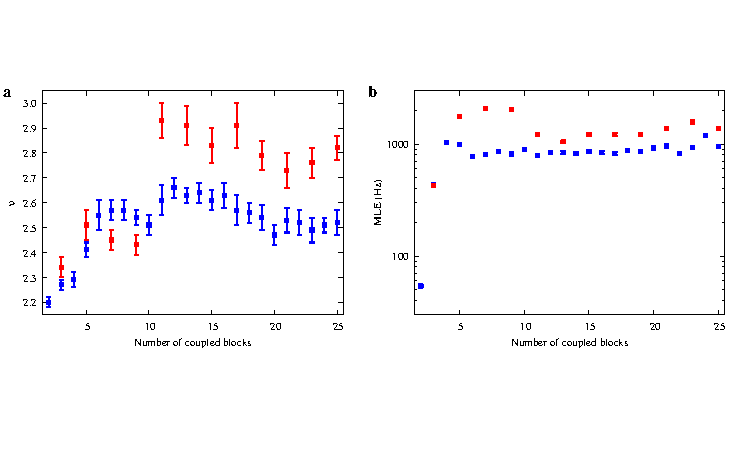
\includegraphics[width=\linewidth,trim={0 1.5cm 0 1.3cm},clip]
    {../blocks/data/nu_mle_blocks.pdf}
    \caption{Boundary (blue) and center (red).}
    \label{fig:nu mle blocks}
\end{figure}

\clearpage

\section{Attractor plots}

\begin{figure}
    \centering
    \begin{minipage}{.47\textwidth}
        \begin{subfigure}{\linewidth}
            \centering
            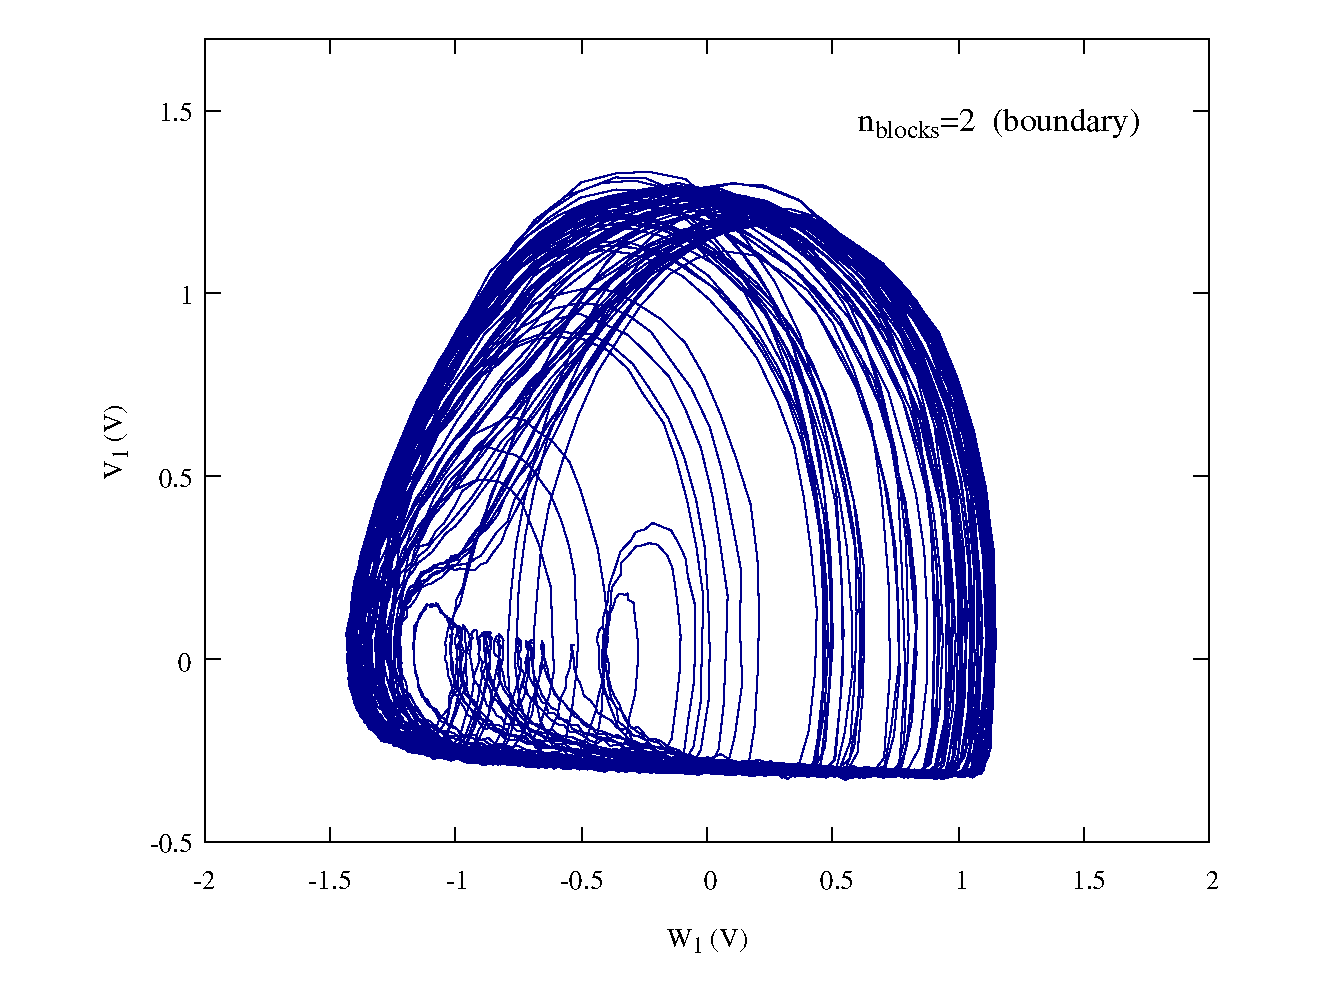
\includegraphics[width=\linewidth]
            {../blocks/2_blocks/attractor.pdf}
        \end{subfigure}
    \end{minipage}
    \begin{minipage}{.47\textwidth}
        \begin{subfigure}{\linewidth}
            \centering
            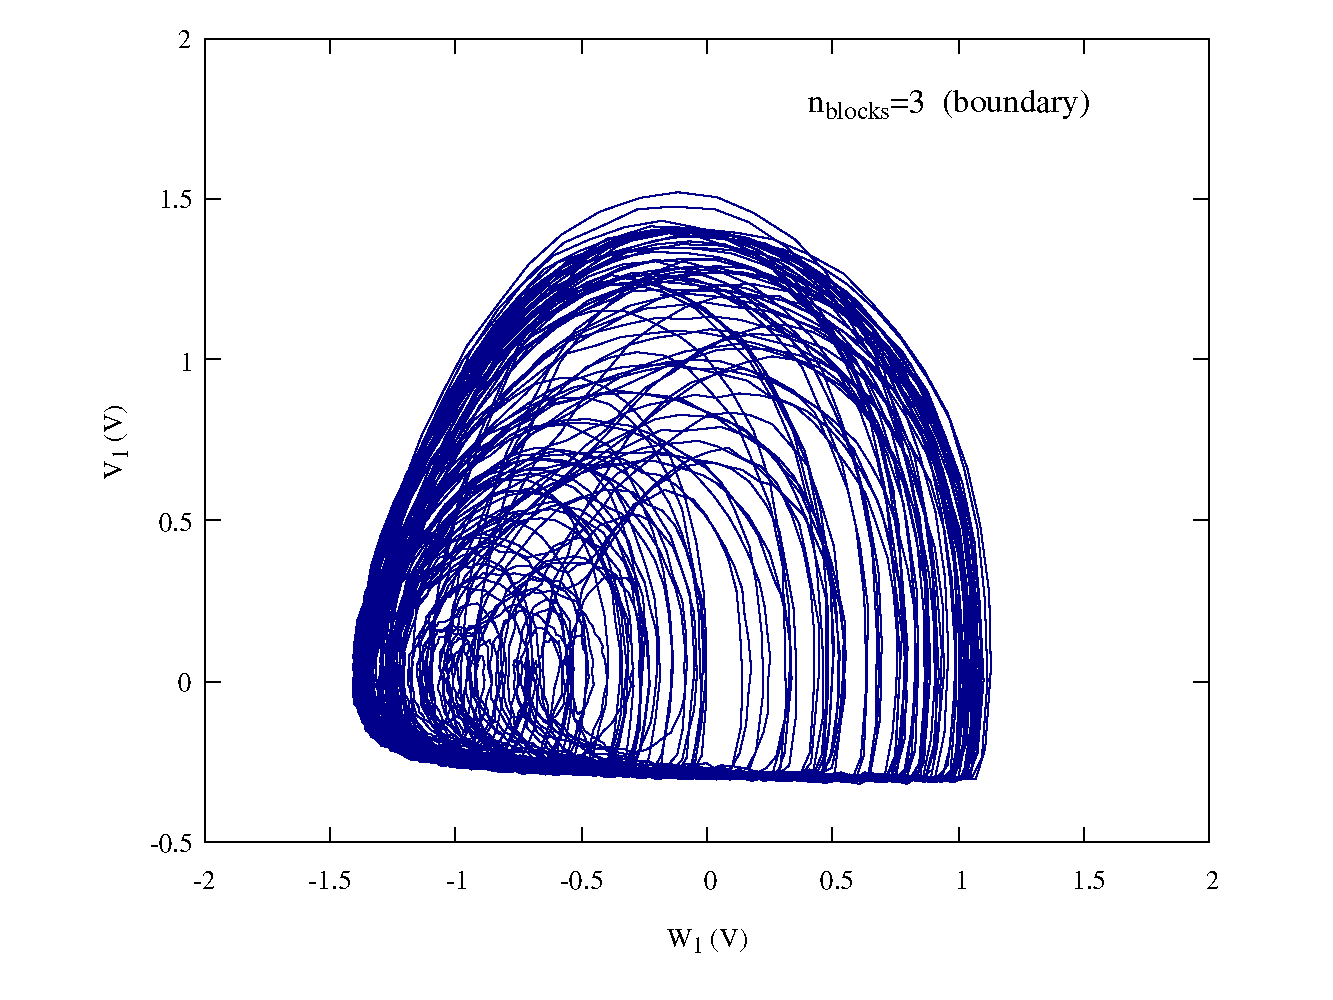
\includegraphics[width=\linewidth]
            {../blocks/3_blocks/edge/attractor.pdf}
        \end{subfigure}
    \end{minipage}
    \begin{minipage}{.47\textwidth}
        \begin{subfigure}{\linewidth}
            \centering
            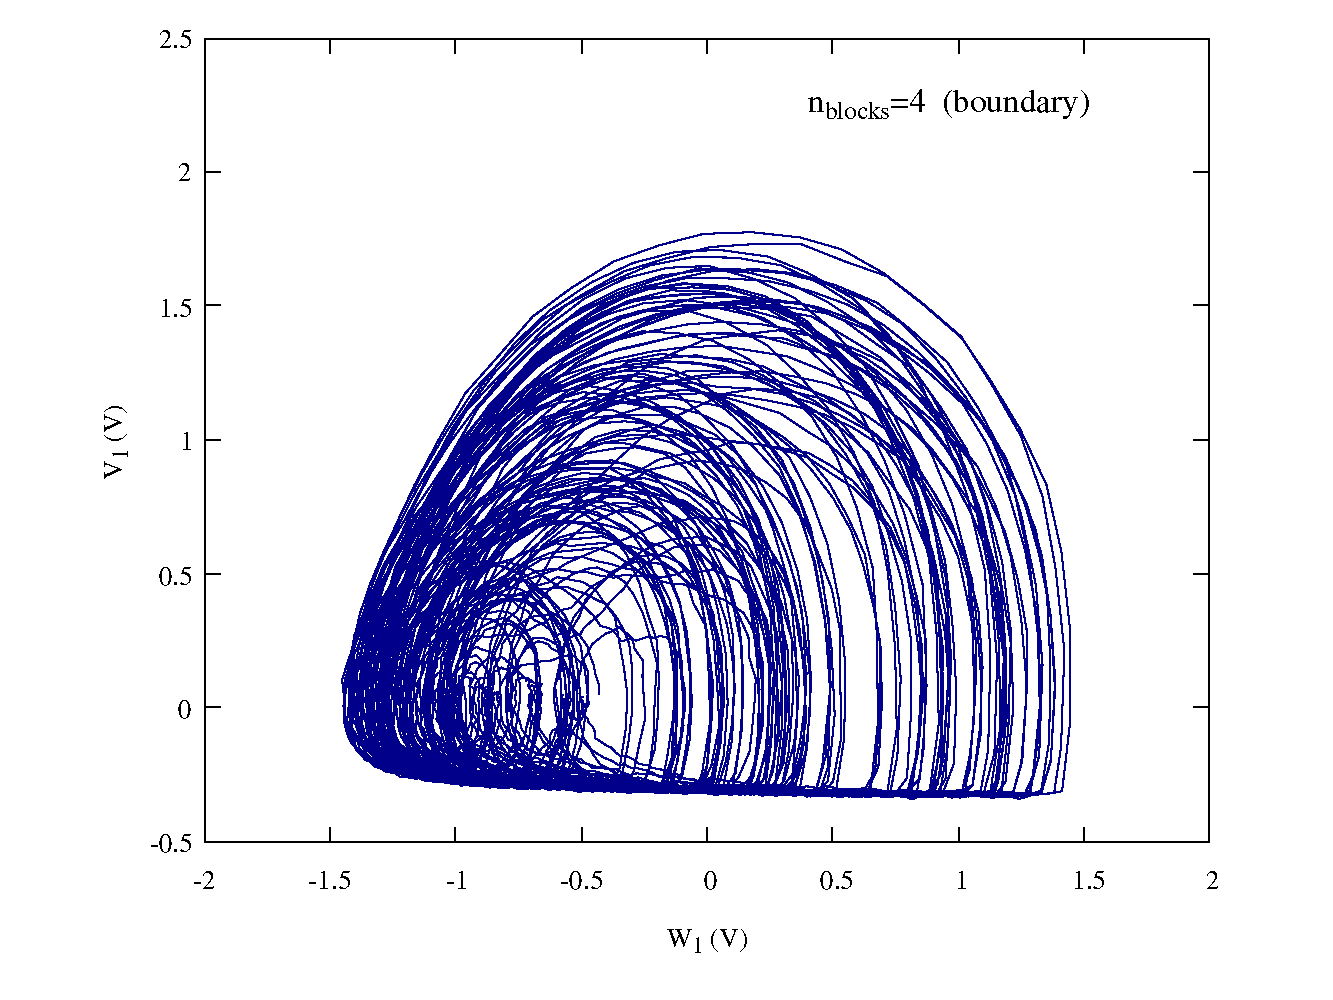
\includegraphics[width=\linewidth]
            {../blocks/4_blocks/attractor.pdf}
        \end{subfigure}
    \end{minipage}
    \begin{minipage}{.47\textwidth}
        \begin{subfigure}{\linewidth}
            \centering
            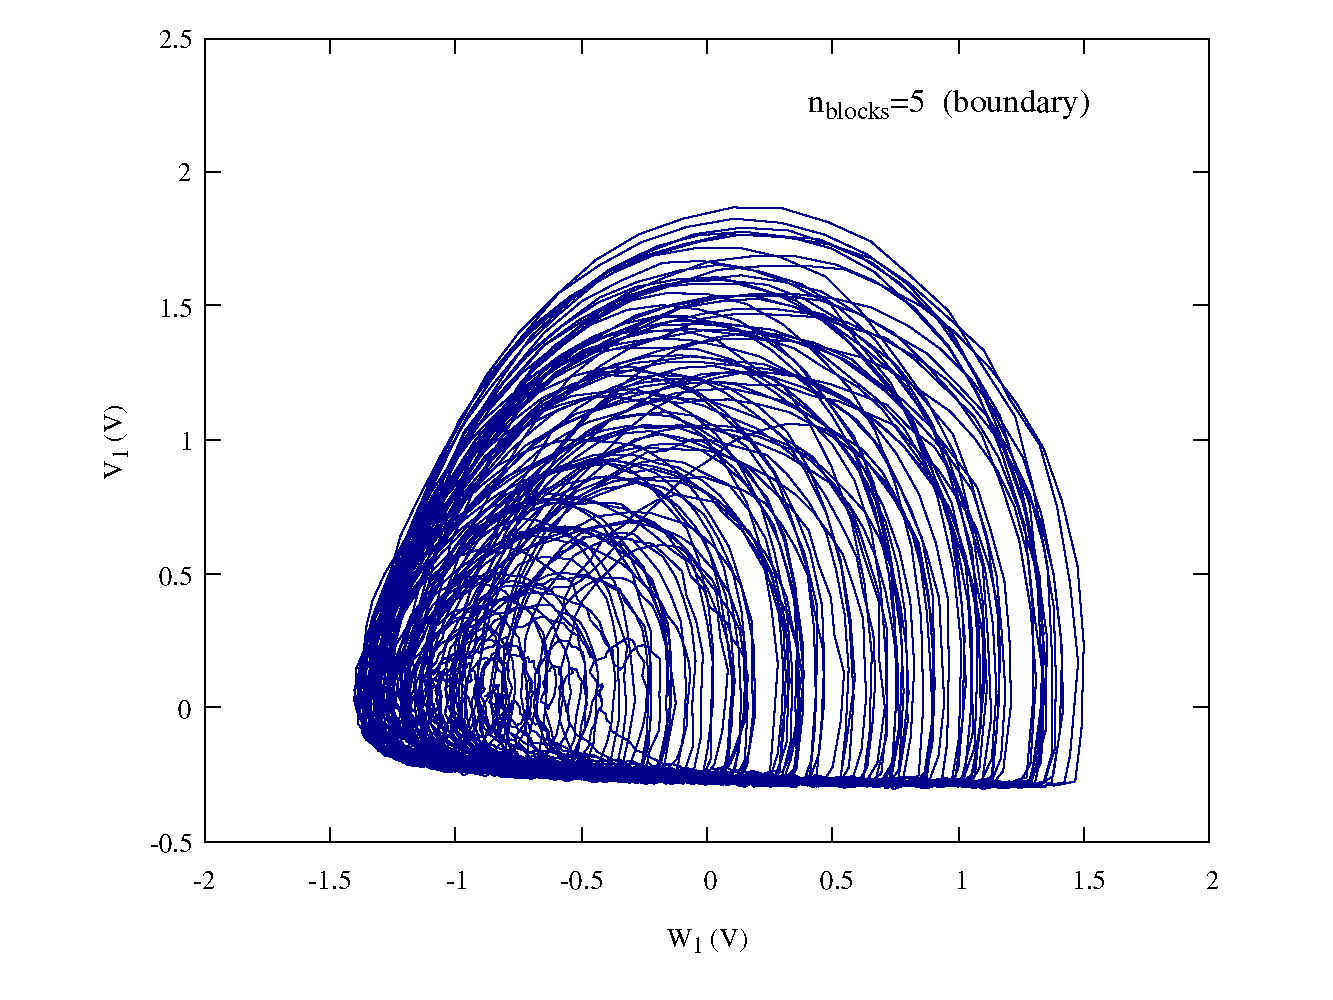
\includegraphics[width=\linewidth]
            {../blocks/5_blocks/edge/attractor.pdf}
        \end{subfigure}
    \end{minipage}
    \begin{minipage}{.47\textwidth}
        \begin{subfigure}{\linewidth}
            \centering
            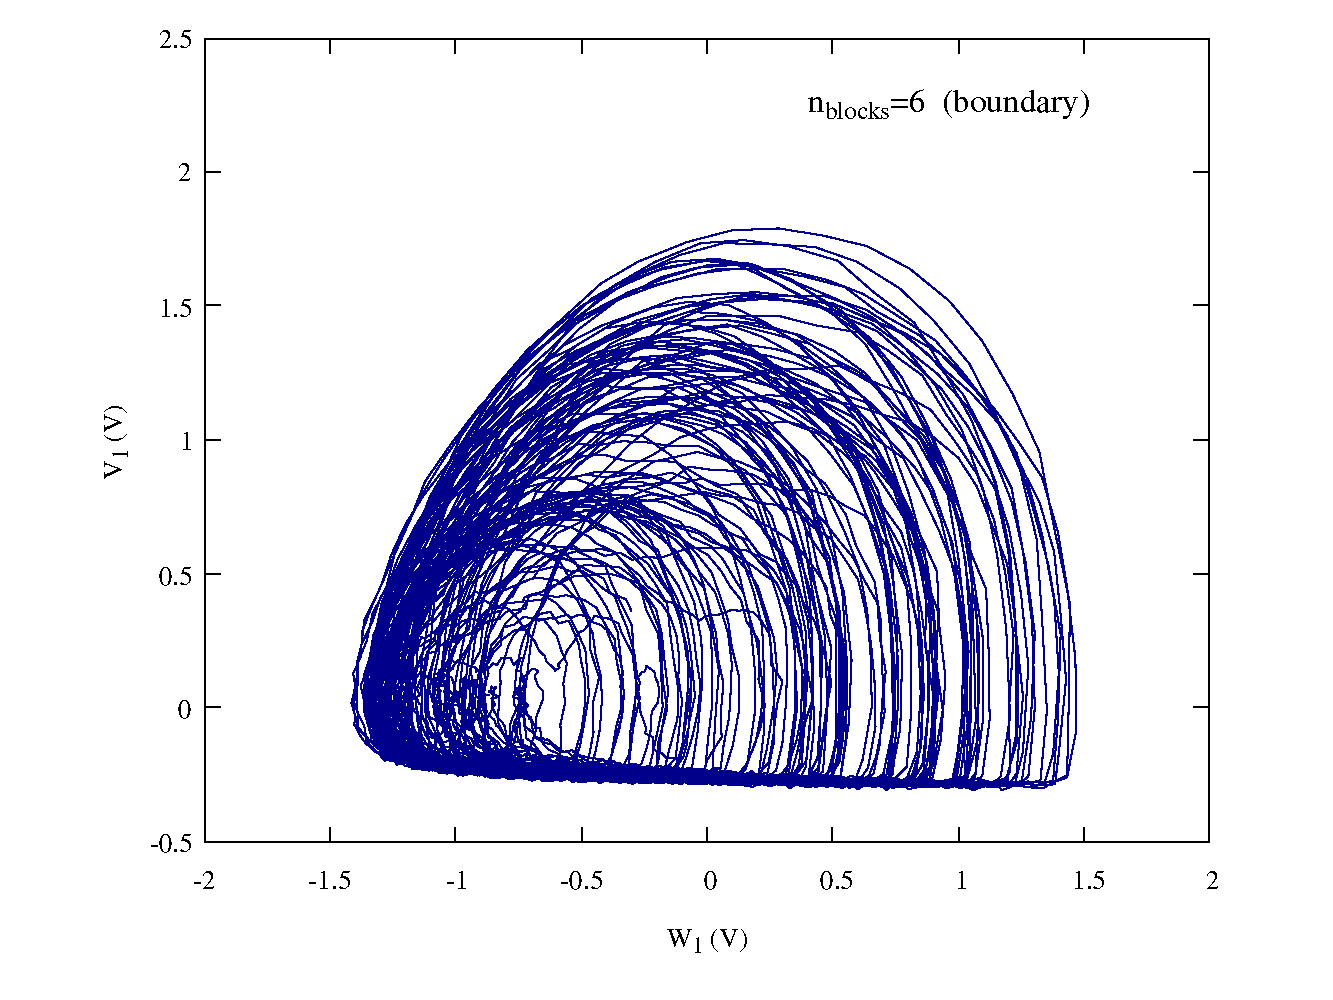
\includegraphics[width=\linewidth]
            {../blocks/6_blocks/attractor.pdf}
        \end{subfigure}
    \end{minipage}
    \begin{minipage}{.47\textwidth}
        \begin{subfigure}{\linewidth}
            \centering
            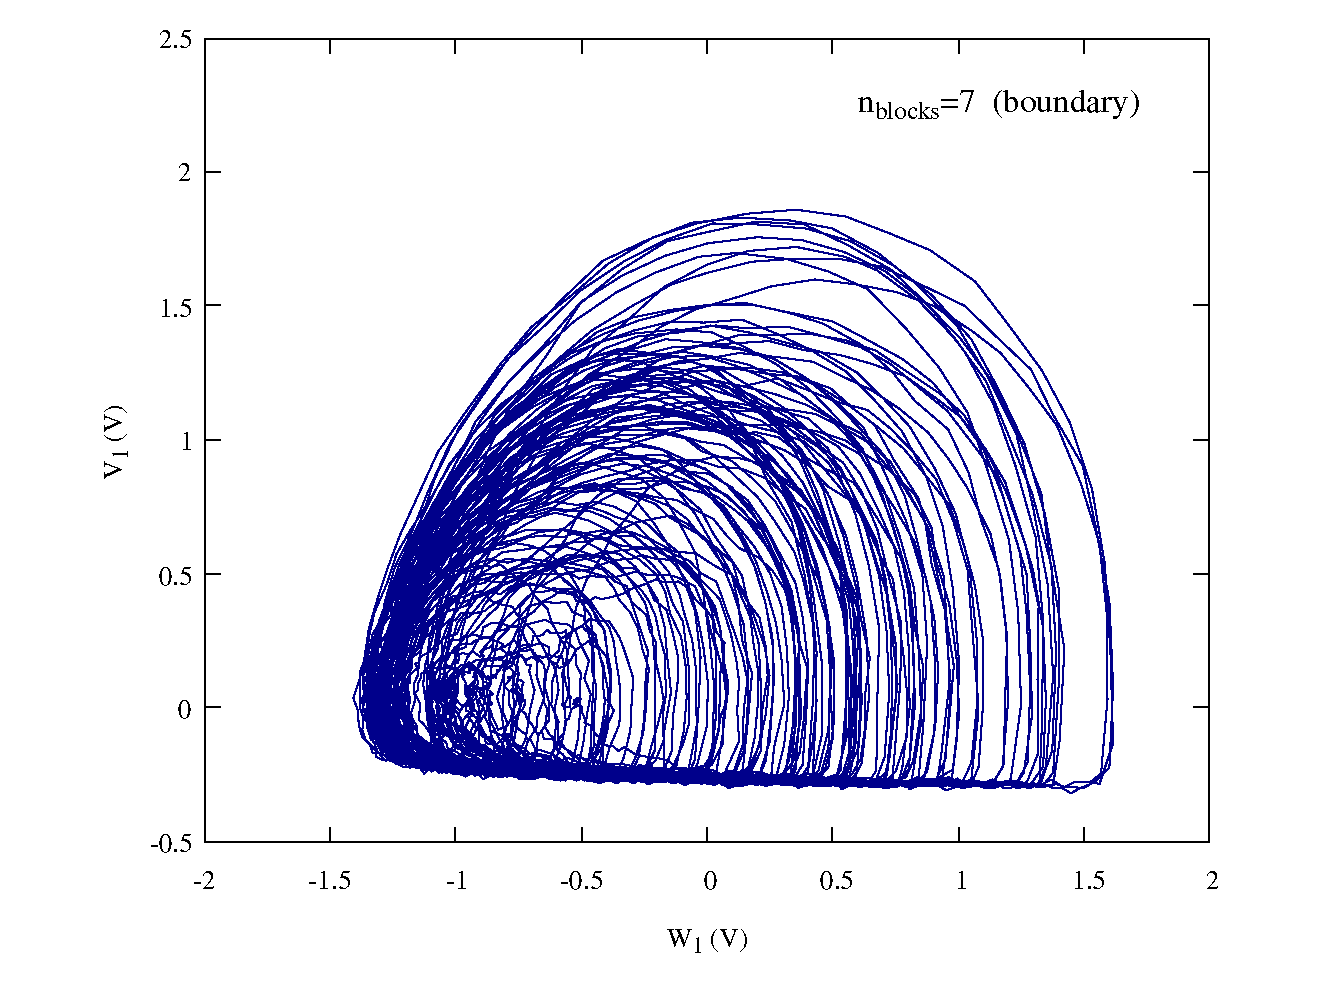
\includegraphics[width=\linewidth]
            {../blocks/7_blocks/edge/attractor.pdf}
        \end{subfigure}
    \end{minipage}
    \begin{minipage}{.47\textwidth}
        \begin{subfigure}{\linewidth}
            \centering
            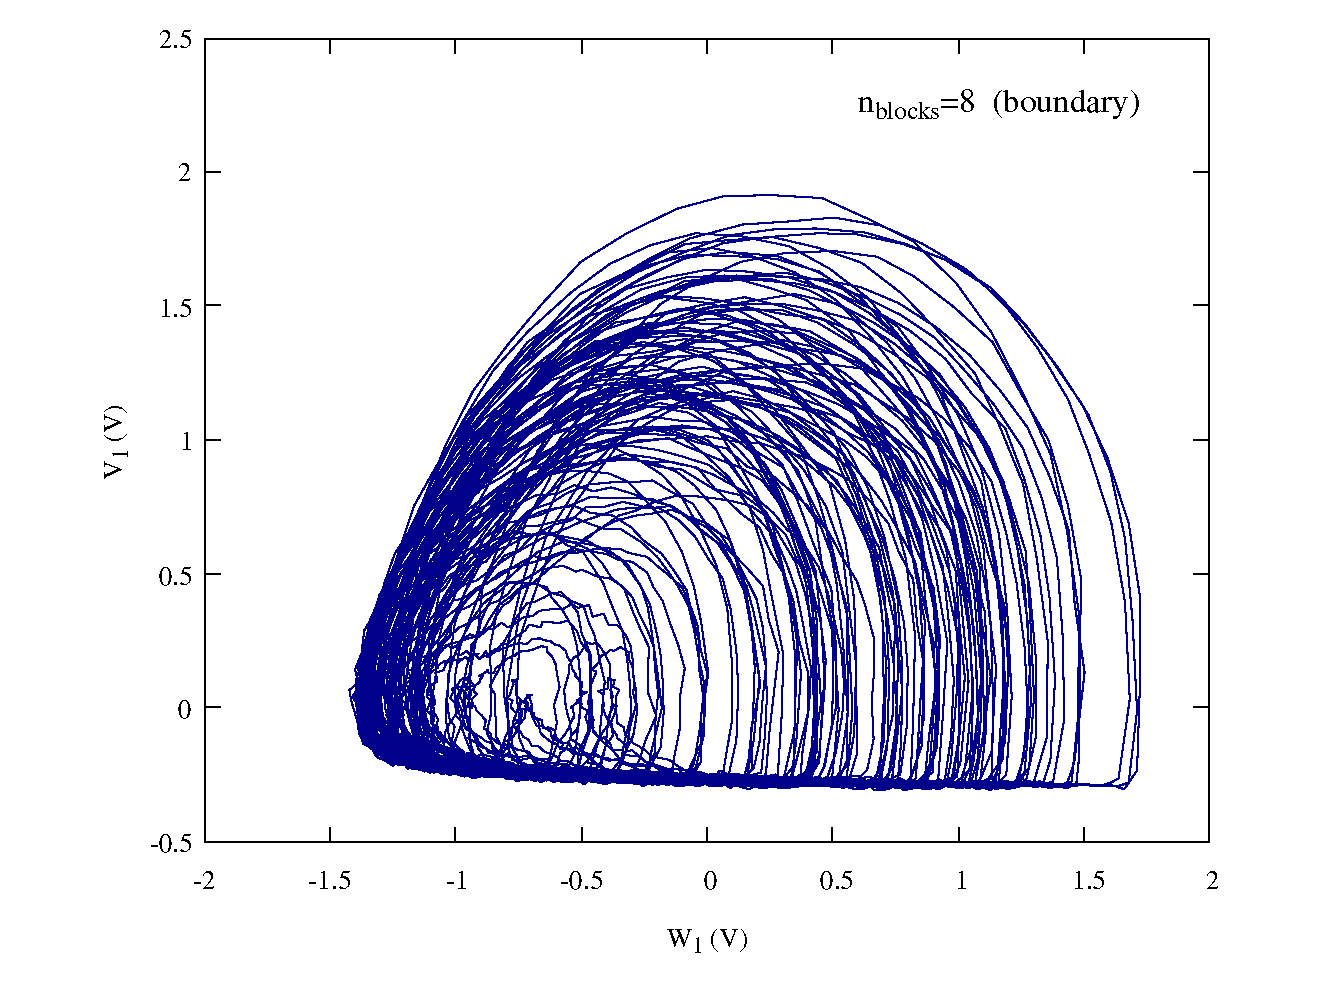
\includegraphics[width=\linewidth]
            {../blocks/8_blocks/attractor.pdf}
        \end{subfigure}
    \end{minipage}
    \begin{minipage}{.47\textwidth}
        \begin{subfigure}{\linewidth}
            \centering
            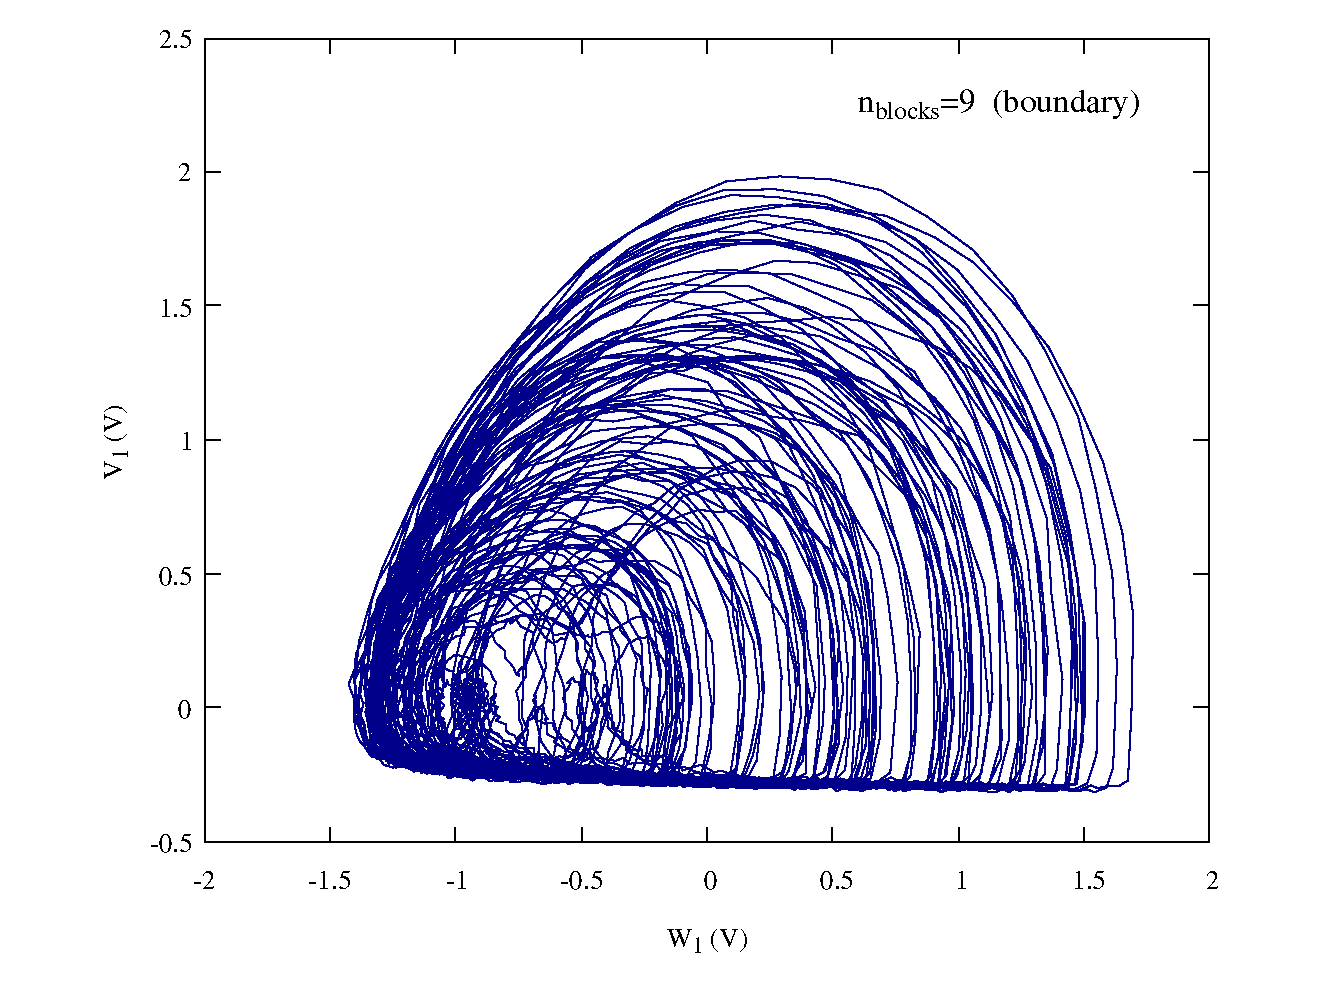
\includegraphics[width=\linewidth]
            {../blocks/9_blocks/edge/attractor.pdf}
        \end{subfigure}
    \end{minipage}
    \caption{Attractors (boundary).}
    \label{fig:attractors 2-9}
\end{figure}

\begin{figure}
    \centering
    \begin{minipage}{.47\textwidth}
        \begin{subfigure}{\linewidth}
            \centering
            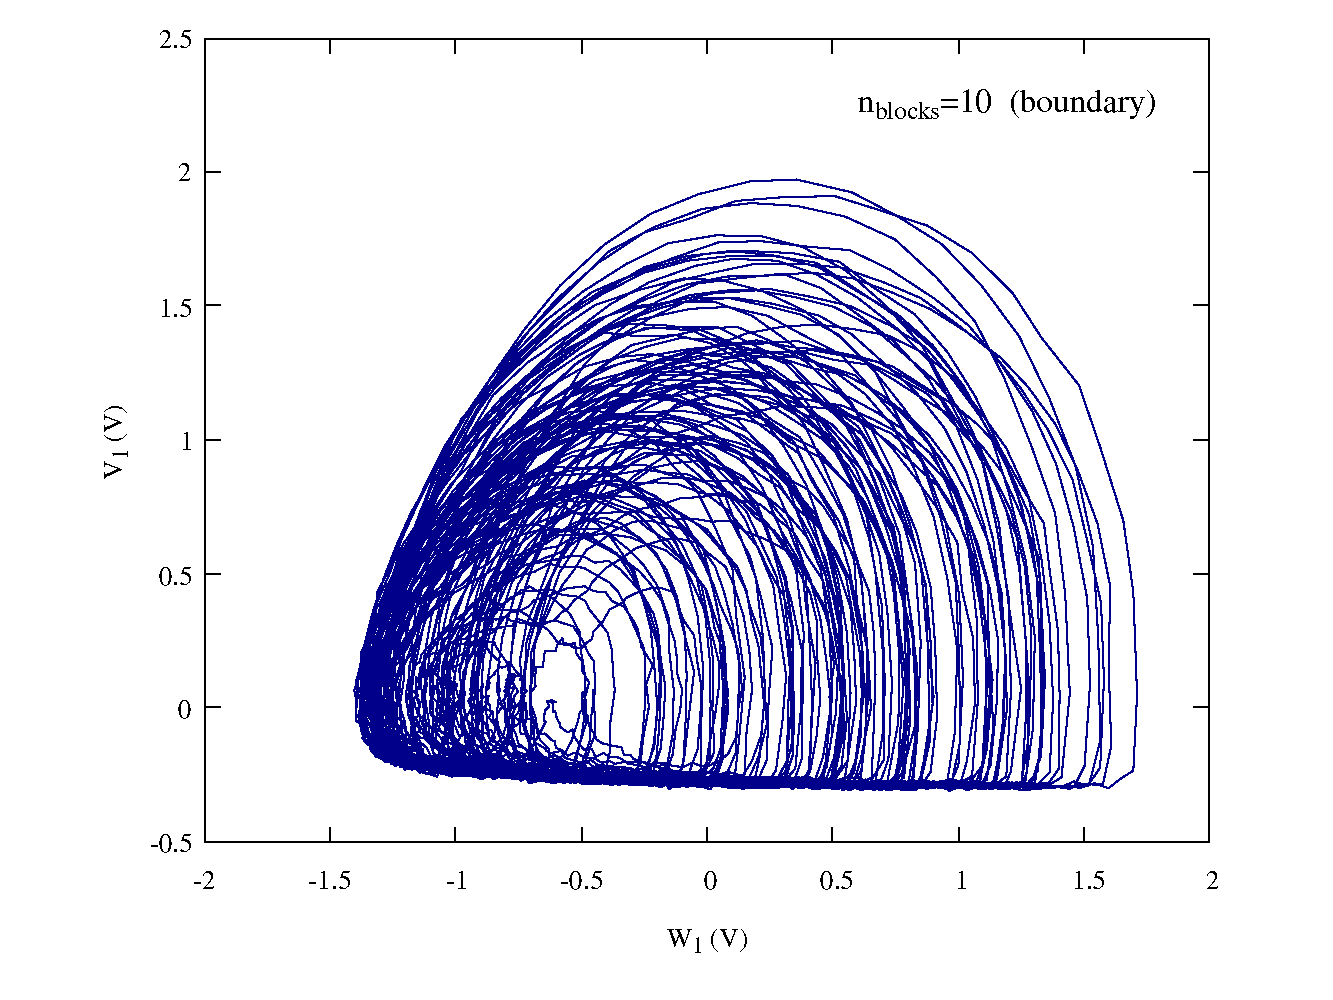
\includegraphics[width=\linewidth]
            {../blocks/10_blocks/attractor.pdf}
        \end{subfigure}
    \end{minipage}
    \begin{minipage}{.47\textwidth}
        \begin{subfigure}{\linewidth}
            \centering
            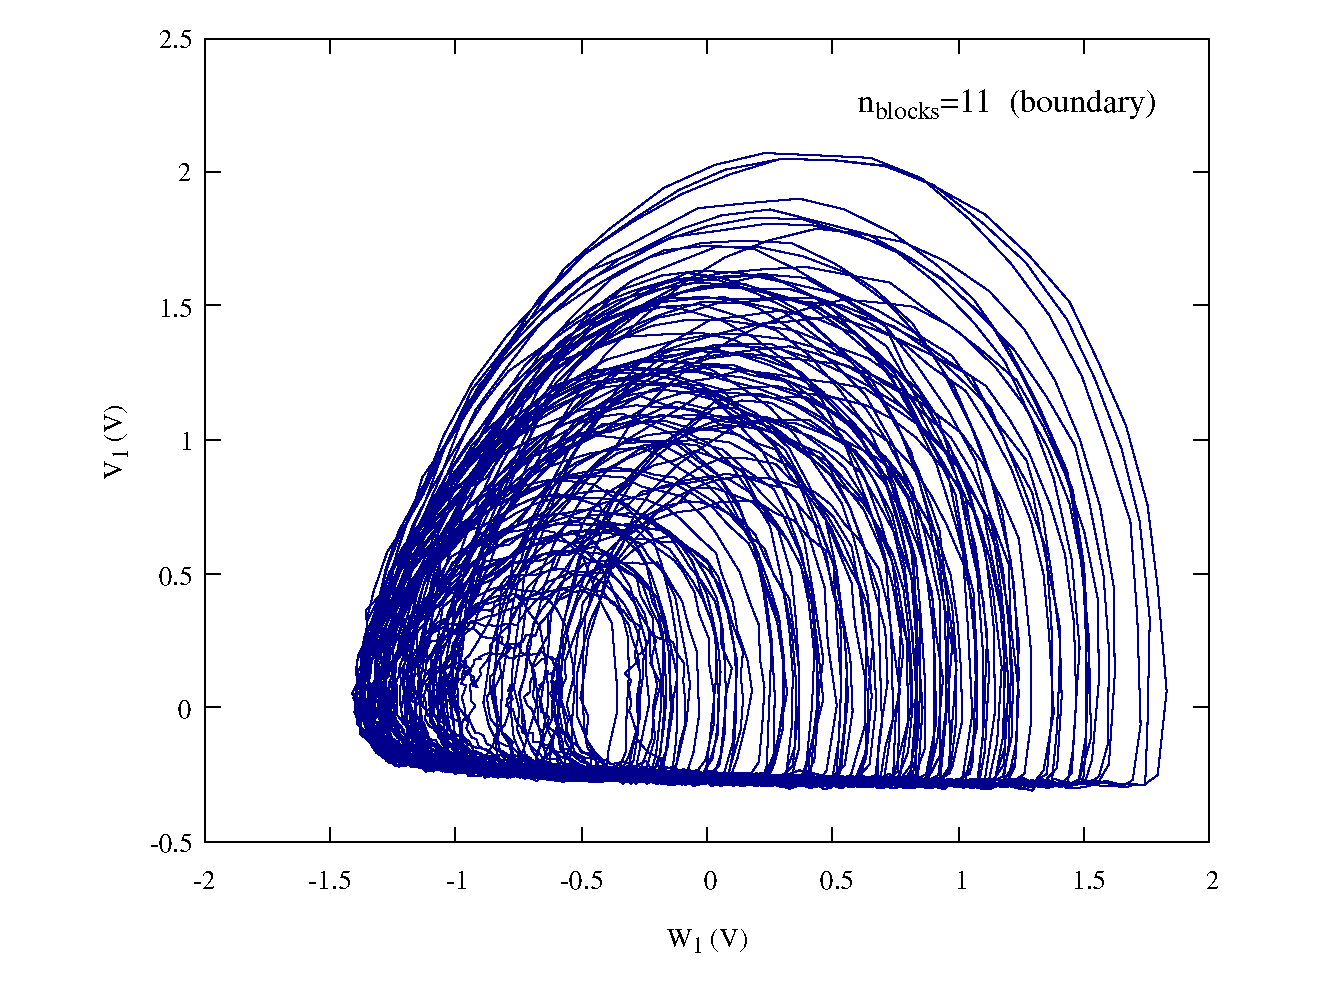
\includegraphics[width=\linewidth]
            {../blocks/11_blocks/edge/attractor.pdf}
        \end{subfigure}
    \end{minipage}
    \begin{minipage}{.47\textwidth}
        \begin{subfigure}{\linewidth}
            \centering
            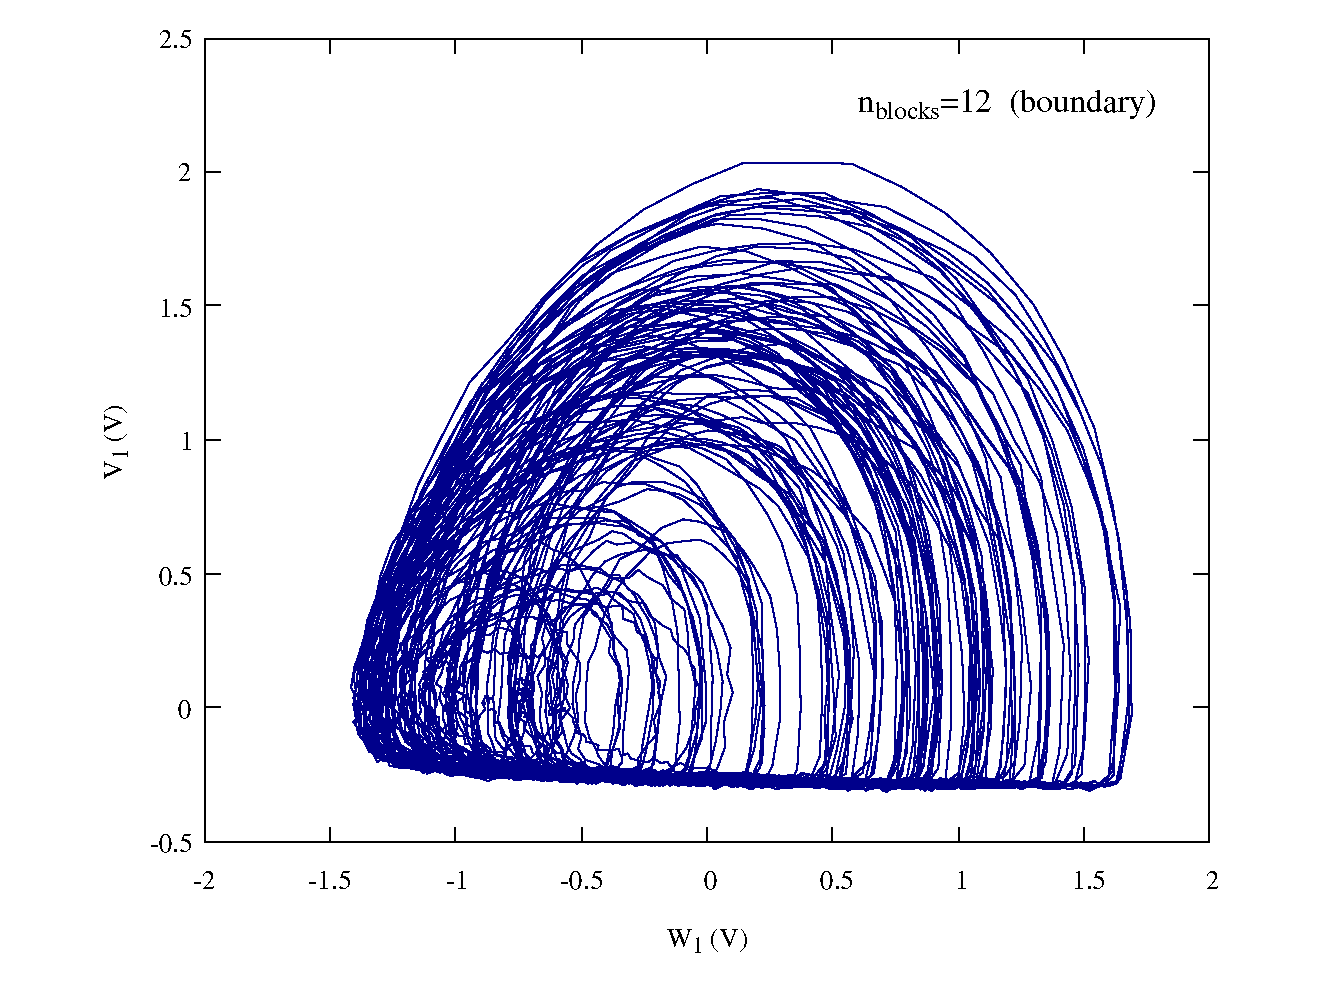
\includegraphics[width=\linewidth]
            {../blocks/12_blocks/attractor.pdf}
        \end{subfigure}
    \end{minipage}
    \begin{minipage}{.47\textwidth}
        \begin{subfigure}{\linewidth}
            \centering
            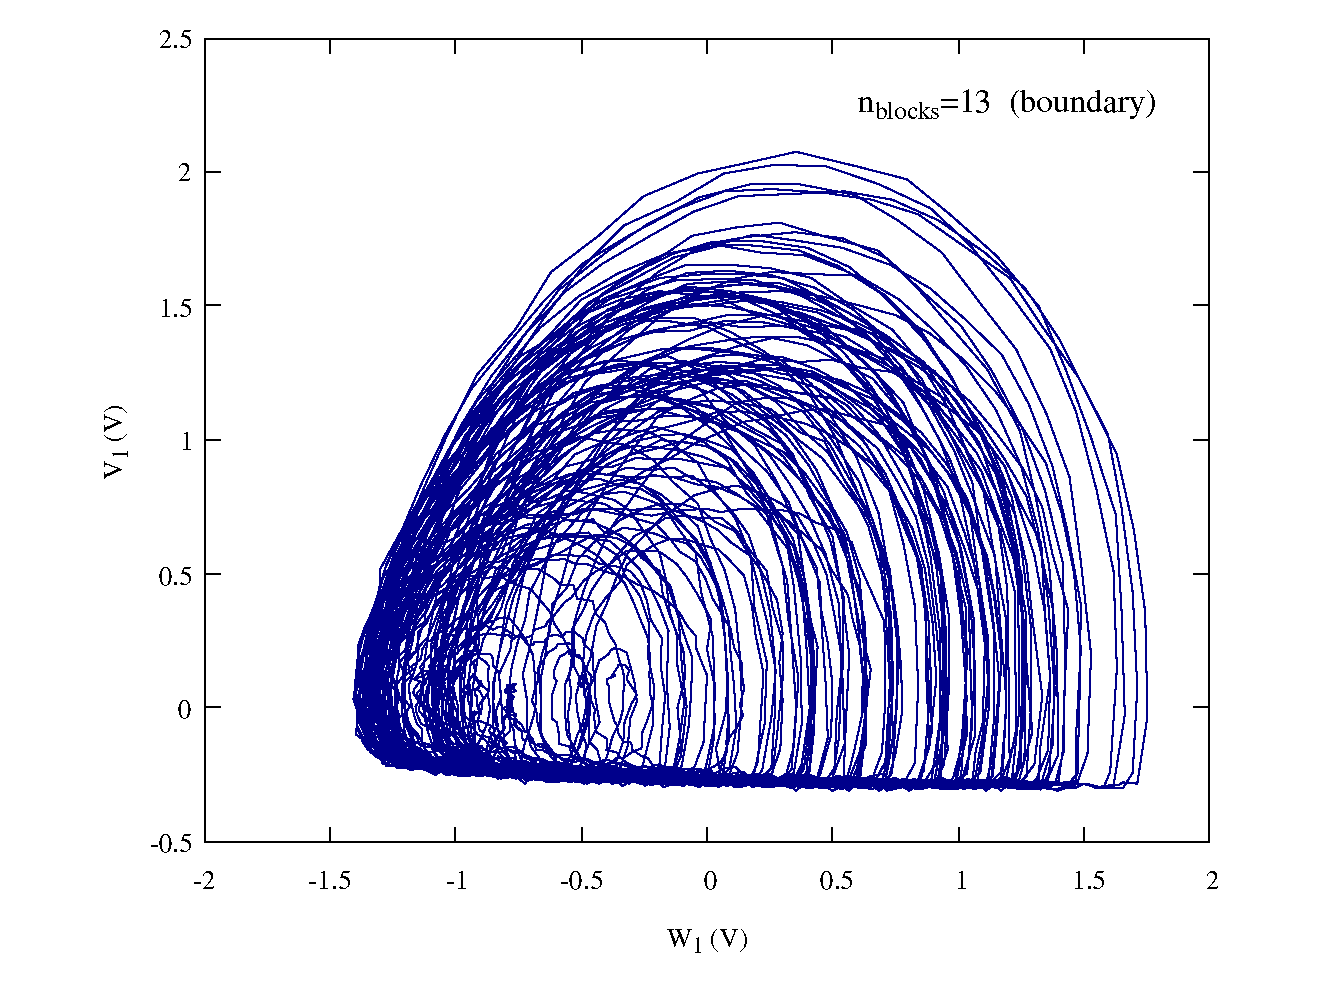
\includegraphics[width=\linewidth]
            {../blocks/13_blocks/edge/attractor.pdf}
        \end{subfigure}
    \end{minipage}
    \begin{minipage}{.47\textwidth}
        \begin{subfigure}{\linewidth}
            \centering
            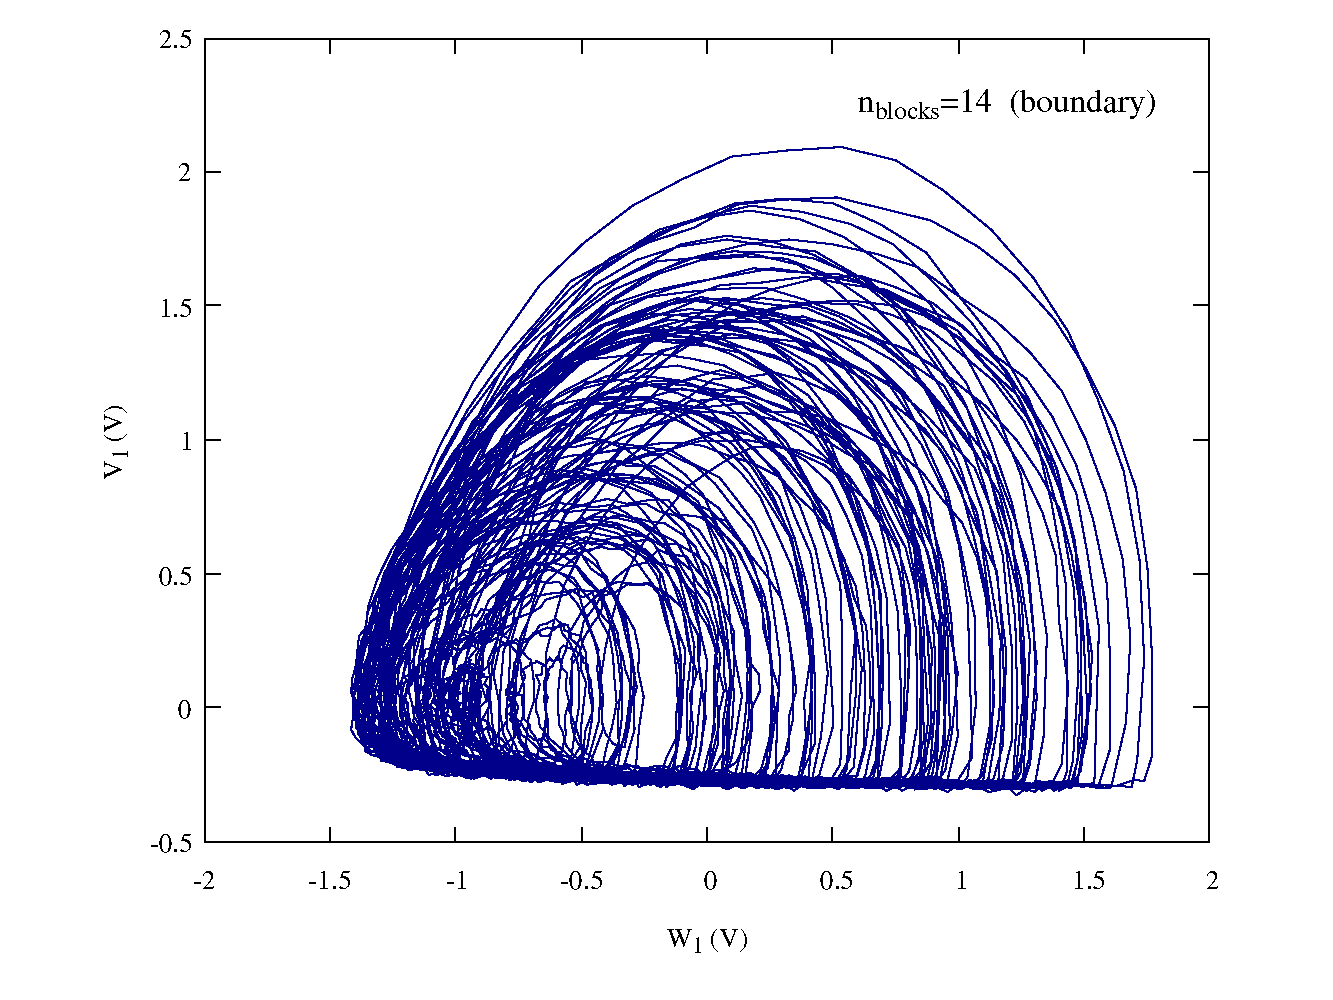
\includegraphics[width=\linewidth]
            {../blocks/14_blocks/attractor.pdf}
        \end{subfigure}
    \end{minipage}
    \begin{minipage}{.47\textwidth}
        \begin{subfigure}{\linewidth}
            \centering
            \includegraphics[width=\linewidth]
            {../blocks/15_blocks/edge/attractor.pdf}
        \end{subfigure}
    \end{minipage}
    \begin{minipage}{.47\textwidth}
        \begin{subfigure}{\linewidth}
            \centering
            \includegraphics[width=\linewidth]
            {../blocks/16_blocks/attractor.pdf}
        \end{subfigure}
    \end{minipage}
    \begin{minipage}{.47\textwidth}
        \begin{subfigure}{\linewidth}
            \centering
            \includegraphics[width=\linewidth]
            {../blocks/17_blocks/edge/attractor.pdf}
        \end{subfigure}
    \end{minipage}
    \caption{Attractors (boundary).}
    \label{fig:attractors 10-17}
\end{figure}

\begin{figure}
    \centering
    \begin{minipage}{.47\textwidth}
        \begin{subfigure}{\linewidth}
            \centering
            \includegraphics[width=\linewidth]
            {../blocks/18_blocks/attractor.pdf}
        \end{subfigure}
    \end{minipage}
    \begin{minipage}{.47\textwidth}
        \begin{subfigure}{\linewidth}
            \centering
            \includegraphics[width=\linewidth]
            {../blocks/19_blocks/edge/attractor.pdf}
        \end{subfigure}
    \end{minipage}
    \begin{minipage}{.47\textwidth}
        \begin{subfigure}{\linewidth}
            \centering
            \includegraphics[width=\linewidth]
            {../blocks/20_blocks/attractor.pdf}
        \end{subfigure}
    \end{minipage}
    \begin{minipage}{.47\textwidth}
        \begin{subfigure}{\linewidth}
            \centering
            \includegraphics[width=\linewidth]
            {../blocks/21_blocks/edge/attractor.pdf}
        \end{subfigure}
    \end{minipage}
    \begin{minipage}{.47\textwidth}
        \begin{subfigure}{\linewidth}
            \centering
            \includegraphics[width=\linewidth]
            {../blocks/22_blocks/attractor.pdf}
        \end{subfigure}
    \end{minipage}
    \begin{minipage}{.47\textwidth}
        \begin{subfigure}{\linewidth}
            \centering
            \includegraphics[width=\linewidth]
            {../blocks/23_blocks/edge/attractor.pdf}
        \end{subfigure}
    \end{minipage}
    \begin{minipage}{.47\textwidth}
        \begin{subfigure}{\linewidth}
            \centering
            \includegraphics[width=\linewidth]
            {../blocks/24_blocks/attractor.pdf}
        \end{subfigure}
    \end{minipage}
    \begin{minipage}{.47\textwidth}
        \begin{subfigure}{\linewidth}
            \centering
            \includegraphics[width=\linewidth]
            {../blocks/25_blocks/edge/attractor.pdf}
        \end{subfigure}
    \end{minipage}
    \caption{Attractors (boundary).}
    \label{fig:attractors 18-25}
\end{figure}

\begin{figure}
    \centering
    \begin{minipage}{.47\textwidth}
        \begin{subfigure}{\linewidth}
            \centering
            \includegraphics[width=\linewidth]
            {../blocks/3_blocks/middle/attractor.pdf}
        \end{subfigure}
    \end{minipage}
    \begin{minipage}{.47\textwidth}
        \begin{subfigure}{\linewidth}
            \centering
            \includegraphics[width=\linewidth]
            {../blocks/5_blocks/middle/attractor.pdf}
        \end{subfigure}
    \end{minipage}
    \begin{minipage}{.47\textwidth}
        \begin{subfigure}{\linewidth}
            \centering
            \includegraphics[width=\linewidth]
            {../blocks/7_blocks/middle/attractor.pdf}
        \end{subfigure}
    \end{minipage}
    \begin{minipage}{.47\textwidth}
        \begin{subfigure}{\linewidth}
            \centering
            \includegraphics[width=\linewidth]
            {../blocks/9_blocks/middle/attractor.pdf}
        \end{subfigure}
    \end{minipage}
    \begin{minipage}{.47\textwidth}
        \begin{subfigure}{\linewidth}
            \centering
            \includegraphics[width=\linewidth]
            {../blocks/11_blocks/middle/attractor.pdf}
        \end{subfigure}
    \end{minipage}
    \begin{minipage}{.47\textwidth}
        \begin{subfigure}{\linewidth}
            \centering
            \includegraphics[width=\linewidth]
            {../blocks/13_blocks/middle/attractor.pdf}
        \end{subfigure}
    \end{minipage}
    \begin{minipage}{.47\textwidth}
        \begin{subfigure}{\linewidth}
            \centering
            \includegraphics[width=\linewidth]
            {../blocks/15_blocks/middle/attractor.pdf}
        \end{subfigure}
    \end{minipage}
    \begin{minipage}{.47\textwidth}
        \begin{subfigure}{\linewidth}
            \centering
            \includegraphics[width=\linewidth]
            {../blocks/17_blocks/middle/attractor.pdf}
        \end{subfigure}
    \end{minipage}
    \caption{Attractors (center).}
    \label{fig:attractors 3-17 middle}
\end{figure}

\begin{figure}
    \centering
    \begin{minipage}{.47\textwidth}
        \begin{subfigure}{\linewidth}
            \centering
            \includegraphics[width=\linewidth]
            {../blocks/19_blocks/middle/attractor.pdf}
        \end{subfigure}
    \end{minipage}
    \begin{minipage}{.47\textwidth}
        \begin{subfigure}{\linewidth}
            \centering
            \includegraphics[width=\linewidth]
            {../blocks/21_blocks/middle/attractor.pdf}
        \end{subfigure}
    \end{minipage}
    \begin{minipage}{.47\textwidth}
        \begin{subfigure}{\linewidth}
            \centering
            \includegraphics[width=\linewidth]
            {../blocks/23_blocks/middle/attractor.pdf}
        \end{subfigure}
    \end{minipage}
    \begin{minipage}{.47\textwidth}
        \begin{subfigure}{\linewidth}
            \centering
            \includegraphics[width=\linewidth]
            {../blocks/25_blocks/middle/attractor.pdf}
        \end{subfigure}
    \end{minipage}
    \caption{Attractors (center).}
    \label{fig:attractors 19-25 middle}
\end{figure}